\pdfminorversion=6 % this is needed to be able to include pdf 1.6. 
                    % For some reasons some old HPSG proceedings have pdf 1.6
\documentclass[11pt,a4paper,fleqn]{article}
\usepackage{times}
\thispagestyle{empty}



\usepackage[T1]{fontenc}   % Silbentrennung

\usepackage[utf8x]{inputenc}
                                                                                                                             
\hyphenation{Acad-e-my}

\usepackage[bookmarks=true,bookmarksopen=true,%
breaklinks=true,%
draft=false,plainpages=false,hyperfootnotes=false,%
pdfauthor={Stefan Müller (Editor)},%
pdftitle={Proceedings of the 11th International Conference on Head-Driven Phrase Structure Grammar},%
pdfkeywords={HPSG}%,
pdftex=true%
%ps2pdf=true  %ohne diesen Treiber geht der Zeilenumbruch in URLs
]{hyperref}% for pdf files
\hypersetup{colorlinks=false, pdfborder={0 0 0}}

\usepackage{pdfpages}
\pdfinclusioncopyfonts=1

\newcommand\formatauthor[2]{\begin{tabular}[t]{@{}c@{}}
  {\LARGE#1\strut}\\
  {\small#2\strut}\\
  \rule{\dimexpr0.5\linewidth-1em}{0pt}
  \end{tabular}\xhfill\ignorespaces}
\newcommand\xhfill{\hspace{1em plus 1fill}}

\begin{document}

\begin{center}
{\Large
                {\bfseries Proceedings of the 11th International Conference on\par Head-Driven Phrase Structure Grammar\par}

                \vspace{8ex}

                     Center for Computational Linguistics, Katholieke Universiteit Leuven\\[\baselineskip]

                        Stefan M{\"u}ller (Editor)\\[\baselineskip]

                                2004\\[\baselineskip]

                          CSLI Publications\\[\baselineskip]

              http://csli-publications.stanford.edu/HPSG/2004 \\[4\baselineskip]

The papers are published under a \href{http://creativecommons.org/licenses/by/4.0/}{CC-BY license}:\\[3pt]
\href{http://creativecommons.org/licenses/by/4.0/}{http://creativecommons.org/licenses/by/4.0/}
}
\end{center}
\newpage
\tableofcontents

\newpage

\section{Editor's Note}
%% -*- coding:utf-8 -*-
The 11th International Conference on Head-Driven Phrase Structure Grammar (2004) was held at
the Center for Computational Linguistics, Katholieke Universiteit Leuven in Belgium.

The conference featured 3 invited talks, 20 papers, and 1 alternate paper,
selected by the program committee (Gosse Bouma, Jonathan Ginzburg, Jong-Bok Kim, Tibor Kiss, Kordula de Kuthy, Bob Levine, Rob Malouf, Philip Miller, Paola Monachesi, Stefan Müller, John Nerbonne, Ivan Sag, Manfred Sailer, Frank Van Eynde, Eun-Jung Yoo, Kei Yoshimoto). 
A workshop on \emph{Semantics in Grammar Engineering} was attached to the conference. It featured one invited talk
and 7 papers, selected by the workshop program committee (Dorothee Beermann, Ash Asudeh, Mary Dalrymple, Markus Egg, Lars Hellan, Jean-Pierre Koenig, Valia Kordoni, Manfred Sailer).

In total there were 32 submissions to the main conference and 7 submissions to the
workshop. 
We want to thank the respective program committees for putting this nice program together.

Thanks go to Frank van Eynde, who was in charge of local arrangements.

As in the past years the contributions to the conference proceedings are based on the five page abstract
that was reviewed by the respective program committees, but there is no additional reviewing of the
longer contribution to the proceedings.
To ensure easy access and fast publication we have chosen an electronic format.

The proceedings include all the papers except those by Farrell Ackerman, Irina Nikolaeva, and Rob Malouf, Ann Copestake, 
Liv Ellingsen, Jonathan Ginzburg, Tibor Kiss, and Adam Przepiórkowski and Alexandr Rosen.


\newpage
\part{Contributions to the Main Conference}
\thispagestyle{empty}
\newpage
        \setcounter{page}{6}
        \phantomsection
        \addcontentsline{toc}{section}{Anne Abeill{\'e}, Olivier Bonami, Dani\`{e}le Godard, Jesse Tseng: The Syntax of French N$'$ Phrases}
\thispagestyle{empty}

\begin{center}
  {\huge\bfseries The Syntax of French N$'$ Phrases\par}

  \bigskip

~\\
\begingroup
\setlength{\leftskip}{0pt plus 1fill}
\setlength{\rightskip}{0pt plus 1fill}
\setlength{\parindent}{0pt}
\setlength{\parfillskip}{0pt}
  \formatauthor{Anne Abeillé}{\begin{tabular}{@{}c@{}}Universite Paris 7\end{tabular}}
\formatauthor{Olivier Bonami}{\begin{tabular}{@{}c@{}}Universite Paris 7\end{tabular}}
\formatauthor{Danièle Godard}{\begin{tabular}{@{}c@{}}Universite Paris 7\end{tabular}}
\formatauthor{Jesse Tseng}{\begin{tabular}{@{}c@{}}Universite Paris 7\end{tabular}}

\par\endgroup

  \vspace*{8ex}

  Proceedings of the 11th International Conference on\par Head-Driven Phrase Structure Grammar

  \bigskip

  Center for Computational Linguistics, Katholieke Universiteit Leuven

  \medskip

  Stefan Müller (Editor)

  \medskip

  2004

  \medskip

  CSLI Publications

  \medskip

  pages 6--26

  \medskip

  \url{http://csli-publications.stanford.edu/HPSG/2004}
\end{center}
\vfill

\noindent



\vfill
\noindent
% APA Style
Abeillé, Anne, Bonami, Olivier, Godard, Danièle, \& Tseng, Jesse. 2004. The Syntax of French N$'$ Phrases. In Müller, Stefan (Ed.), \emph{{Proceedings of the 11th International Conference on Head-Driven Phrase Structure Grammar, Center for Computational Linguistics, Katholieke Universiteit Leuven}}, 6--26. Stanford,
CA: CSLI Publications. \hfill\href{http://creativecommons.org/licenses/by/4.0/}{\includegraphics[height=.75em]{Includes/ccby.eps}}

\newpage
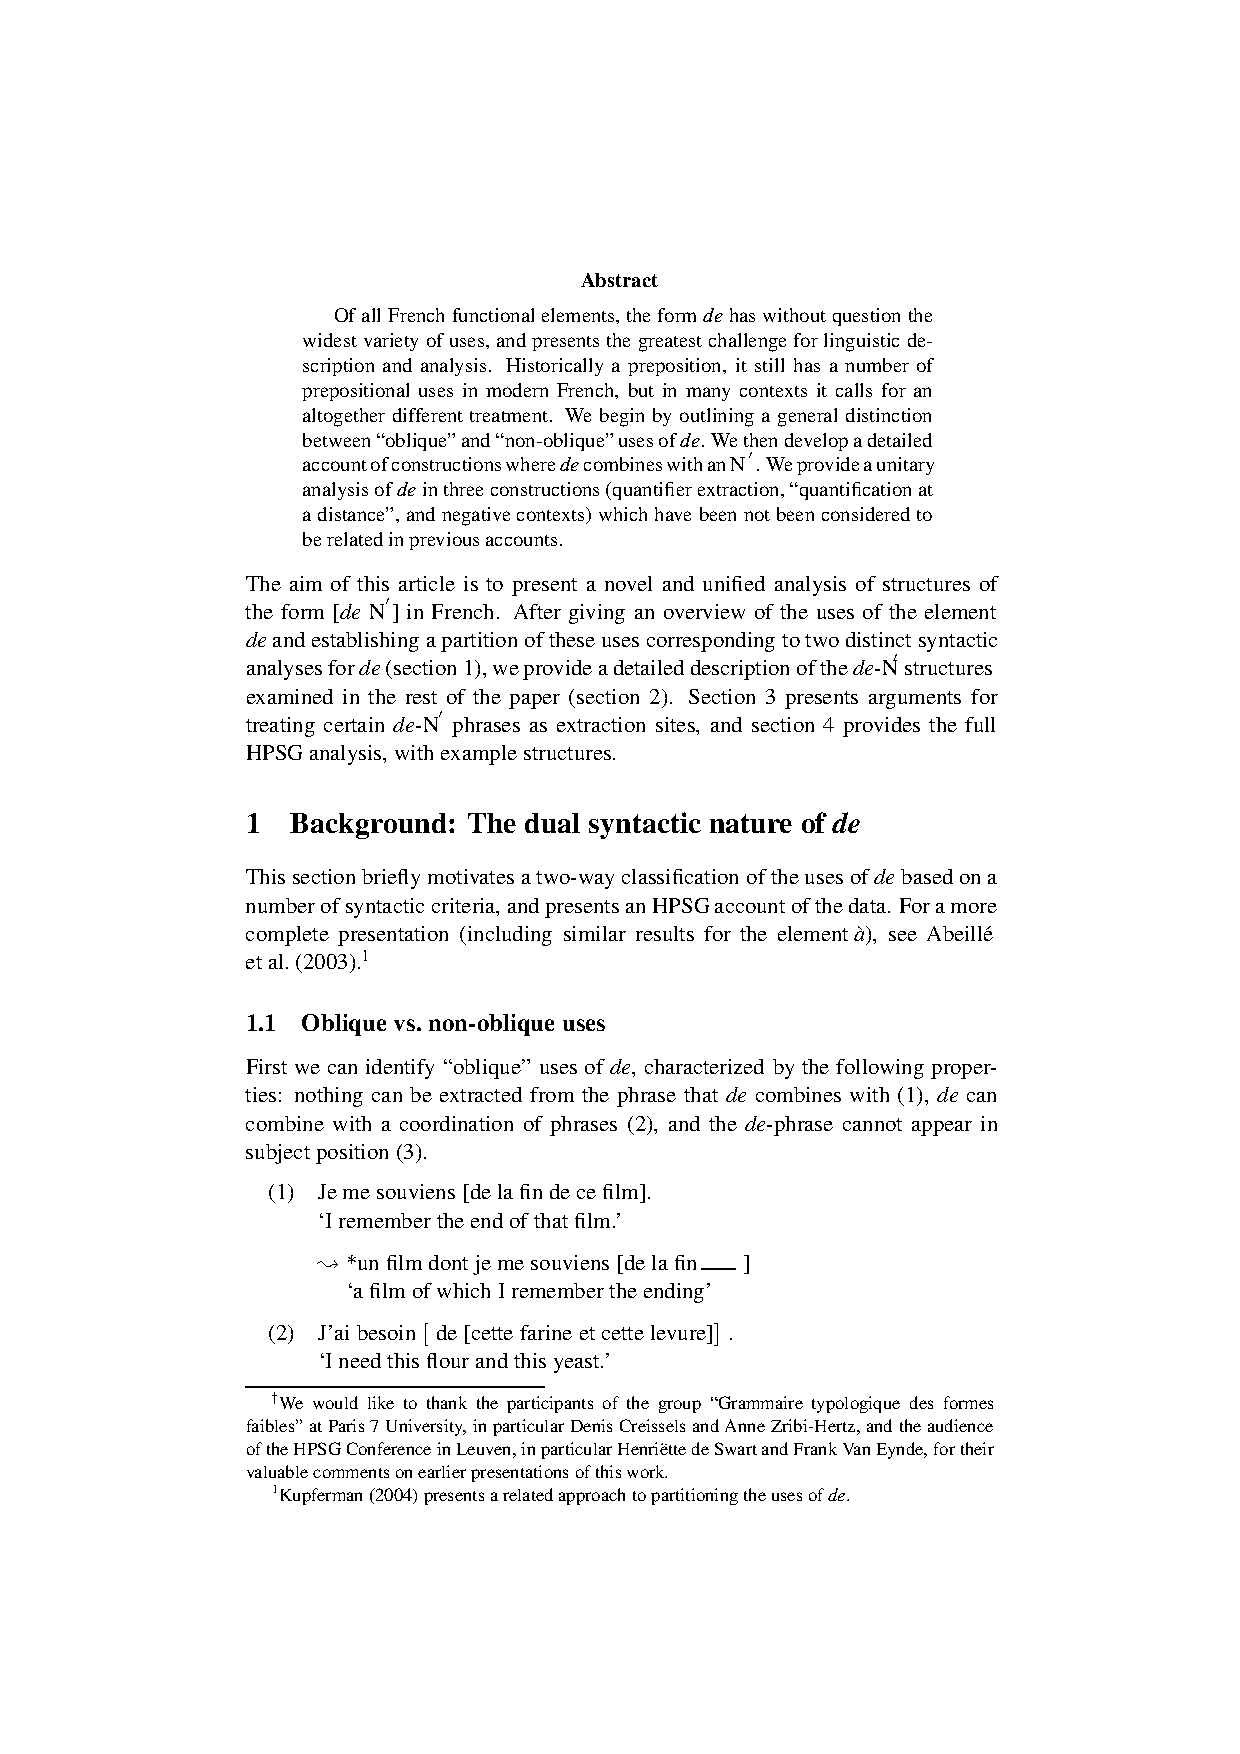
\includepdf[pages=-,pagecommand=\thispagestyle{plain}]{Includes/abgt.pdf}
        \setcounter{page}{27}
        \phantomsection
        \addcontentsline{toc}{section}{Doug Arnold: Non-Restrictive Relative Clauses in Construction Based HPSG}
\thispagestyle{empty}

\begin{center}
  {\huge\bfseries Non-Restrictive Relative Clauses in Construction Based HPSG\par}

  \bigskip

~\\
\begingroup
\setlength{\leftskip}{0pt plus 1fill}
\setlength{\rightskip}{0pt plus 1fill}
\setlength{\parindent}{0pt}
\setlength{\parfillskip}{0pt}
  \formatauthor{Doug Arnold}{\begin{tabular}{@{}c@{}}University of Essex\end{tabular}}

\par\endgroup

  \vspace*{8ex}

  Proceedings of the 11th International Conference on\par Head-Driven Phrase Structure Grammar

  \bigskip

  Center for Computational Linguistics, Katholieke Universiteit Leuven

  \medskip

  Stefan Müller (Editor)

  \medskip

  2004

  \medskip

  CSLI Publications

  \medskip

  pages 27--47

  \medskip

  \url{http://csli-publications.stanford.edu/HPSG/2004}
\end{center}
\vfill

\noindent



\vfill
\noindent
% APA Style
Arnold, Doug. 2004. Non-Restrictive Relative Clauses in Construction Based HPSG. In Müller, Stefan (Ed.), \emph{{Proceedings of the 11th International Conference on Head-Driven Phrase Structure Grammar, Center for Computational Linguistics, Katholieke Universiteit Leuven}}, 27--47. Stanford,
CA: CSLI Publications. \hfill\href{http://creativecommons.org/licenses/by/4.0/}{\includegraphics[height=.75em]{Includes/ccby.eps}}

\newpage
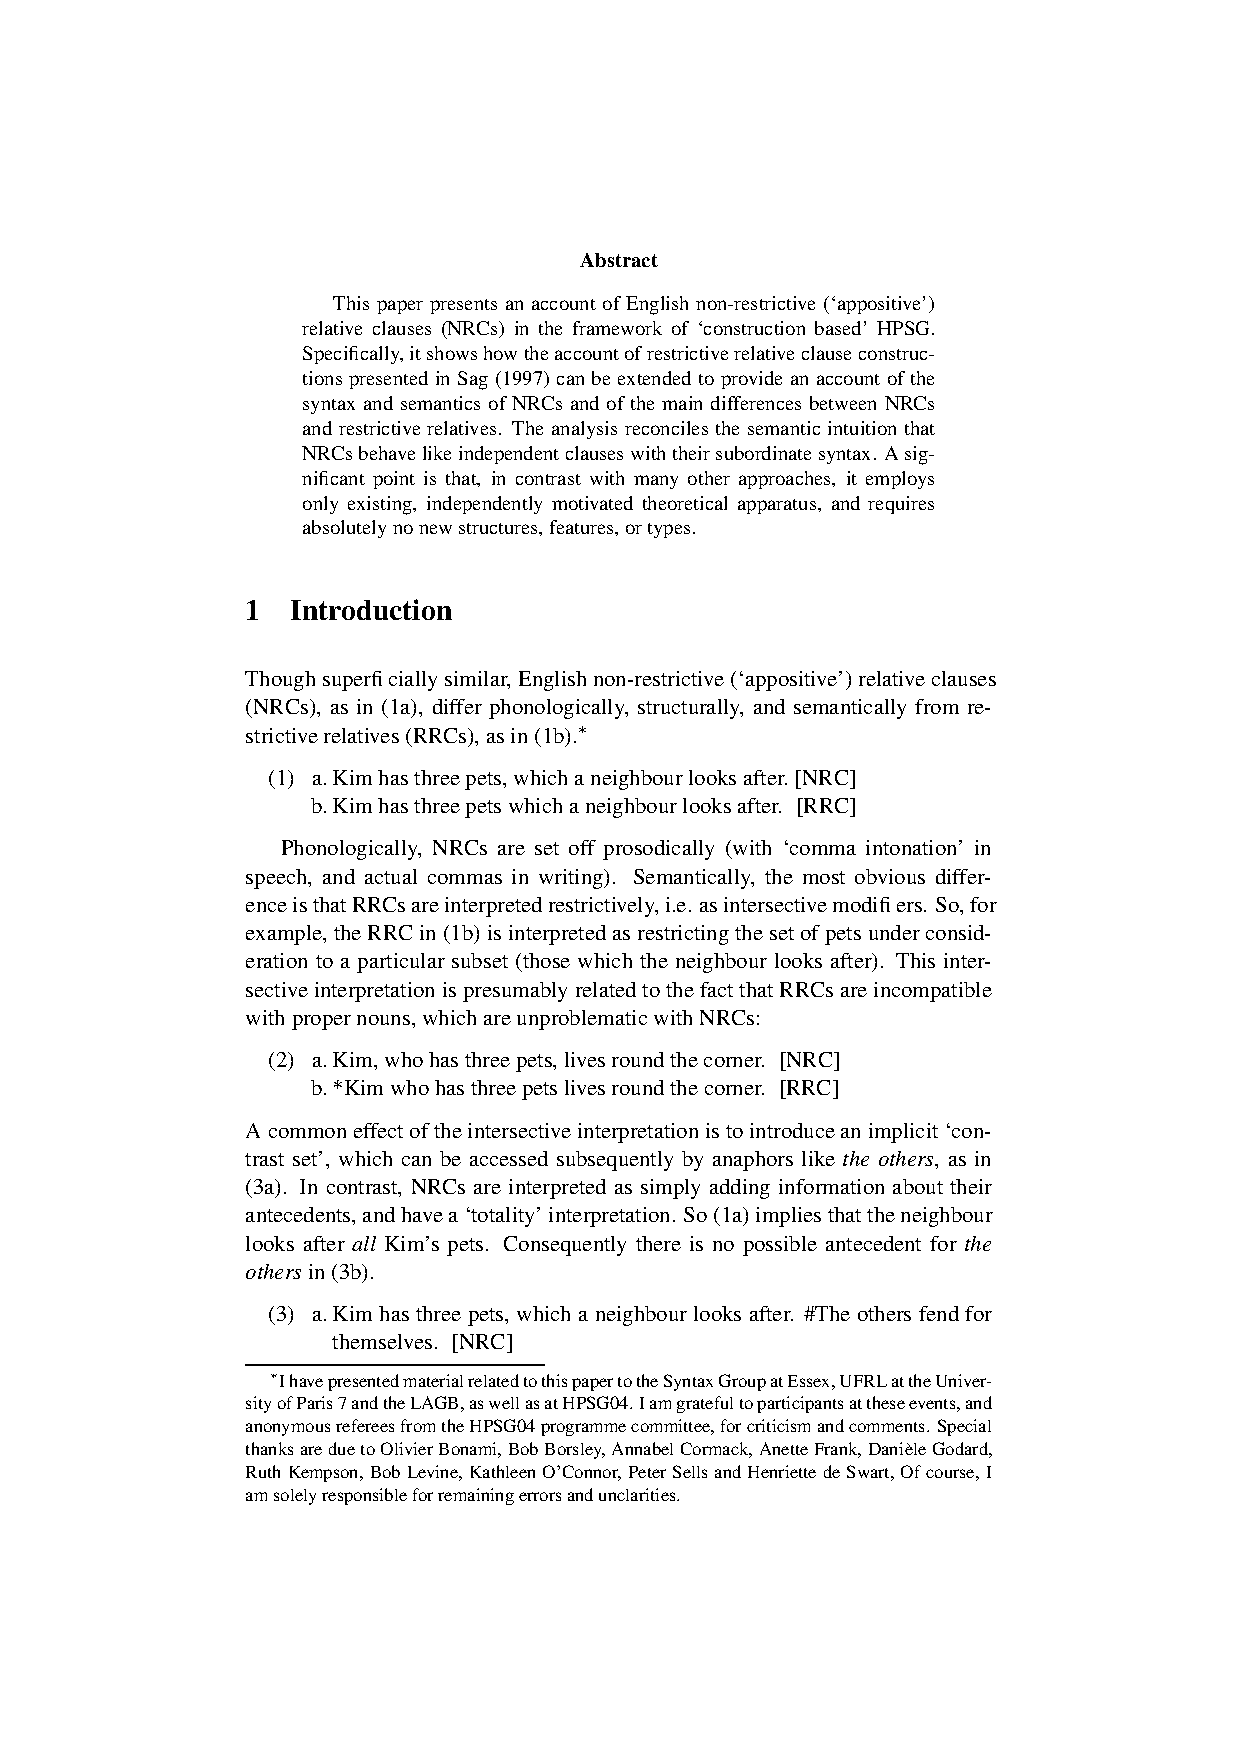
\includepdf[pages=-,pagecommand=\thispagestyle{plain}]{Includes/arnold.pdf}
        \setcounter{page}{48}
        \phantomsection
        \addcontentsline{toc}{section}{John Beavers, Ivan A. Sag: Coordinate Ellipsis and Apparent Non-Constituent Coordination}
\thispagestyle{empty}

\begin{center}
  {\huge\bfseries Coordinate Ellipsis and Apparent Non-Constituent Coordination\par}

  \bigskip

~\\
\begingroup
\setlength{\leftskip}{0pt plus 1fill}
\setlength{\rightskip}{0pt plus 1fill}
\setlength{\parindent}{0pt}
\setlength{\parfillskip}{0pt}
  \formatauthor{John Beavers}{\begin{tabular}{@{}c@{}}University of Texas\end{tabular}}
\formatauthor{Ivan A. Sag}{\begin{tabular}{@{}c@{}}Standford University\end{tabular}}

\par\endgroup

  \vspace*{8ex}

  Proceedings of the 11th International Conference on\par Head-Driven Phrase Structure Grammar

  \bigskip

  Center for Computational Linguistics, Katholieke Universiteit Leuven

  \medskip

  Stefan Müller (Editor)

  \medskip

  2004

  \medskip

  CSLI Publications

  \medskip

  pages 48--69

  \medskip

  \url{http://csli-publications.stanford.edu/HPSG/2004}
\end{center}
\vfill

\noindent



\vfill
\noindent
% APA Style
Beavers, John, \& Sag, Ivan A. 2004. Coordinate Ellipsis and Apparent Non-Constituent Coordination. In Müller, Stefan (Ed.), \emph{{Proceedings of the 11th International Conference on Head-Driven Phrase Structure Grammar, Center for Computational Linguistics, Katholieke Universiteit Leuven}}, 48--69. Stanford,
CA: CSLI Publications. \hfill\href{http://creativecommons.org/licenses/by/4.0/}{\includegraphics[height=.75em]{Includes/ccby.eps}}

\newpage
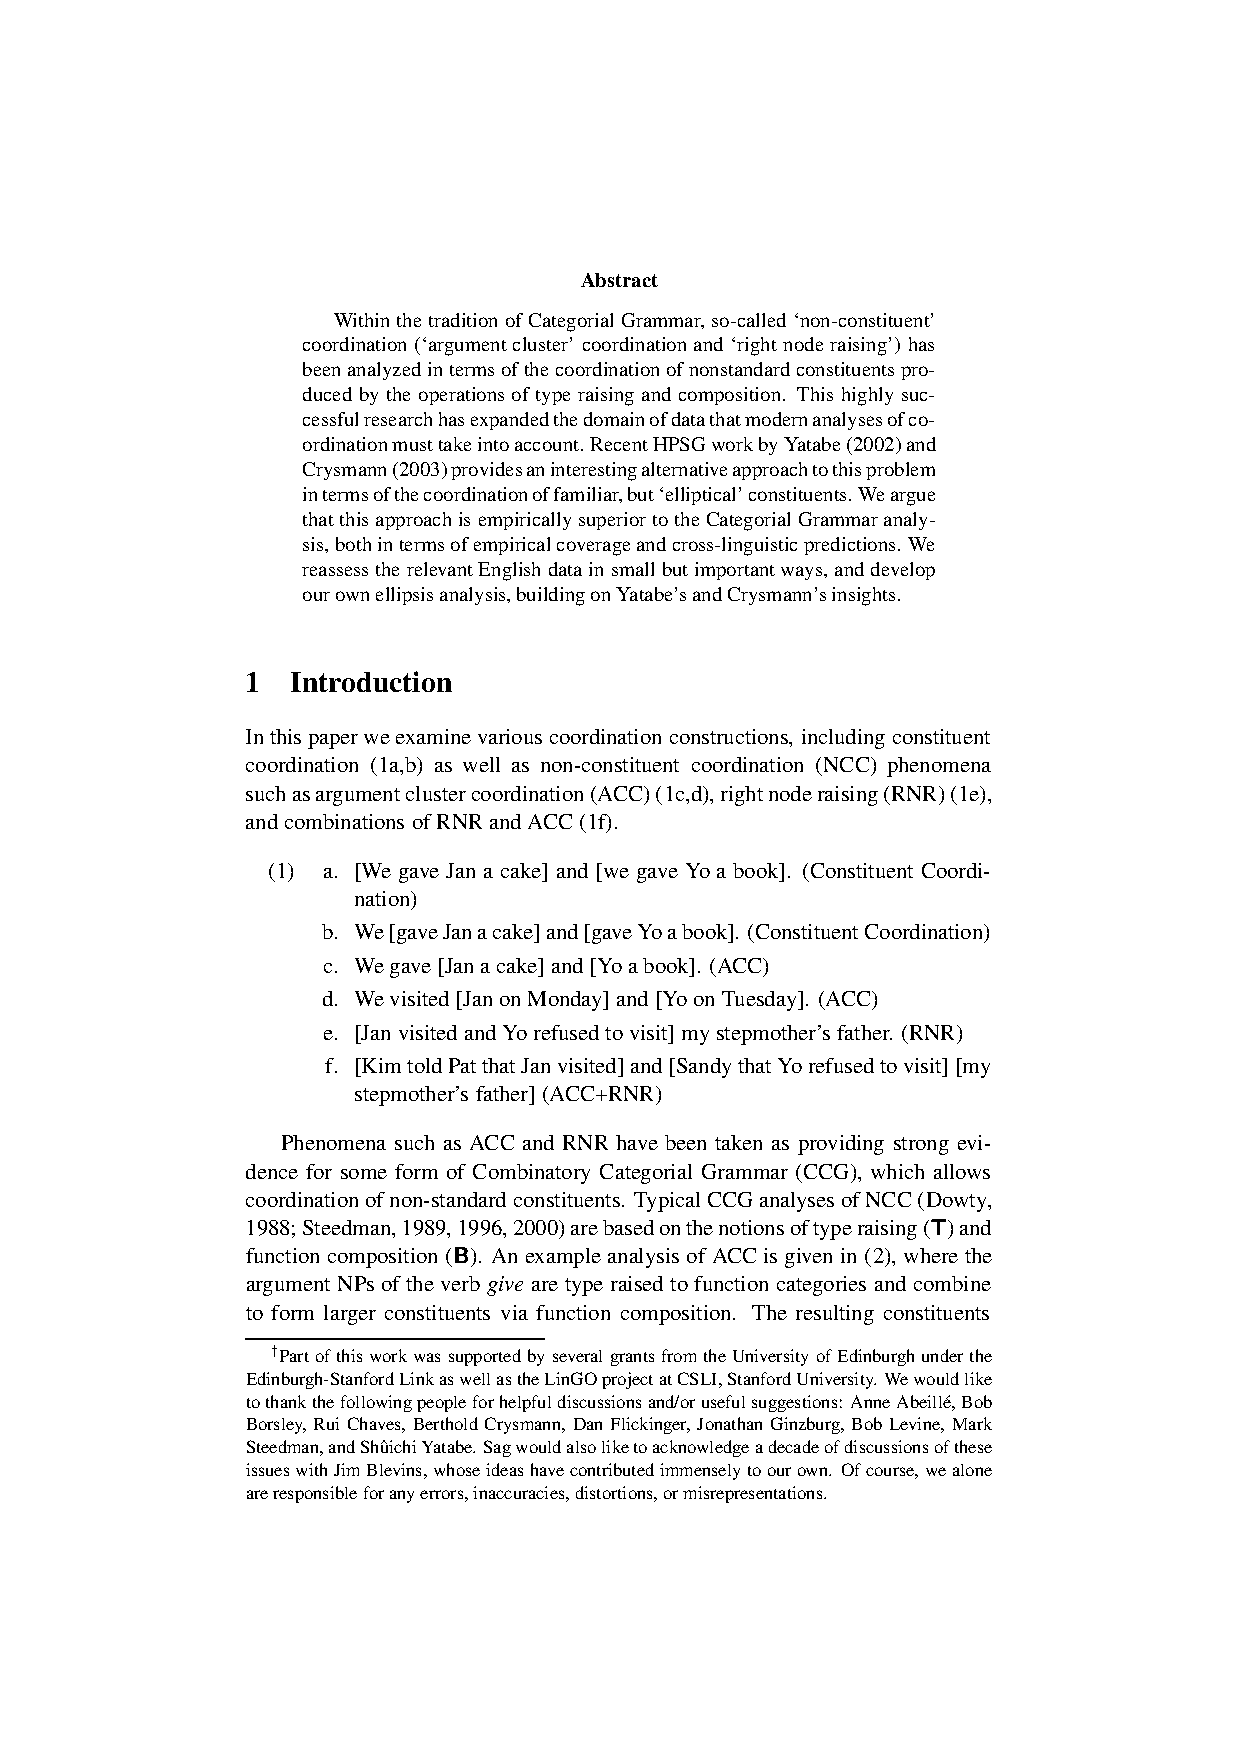
\includepdf[pages=-,pagecommand=\thispagestyle{plain}]{Includes/beavers-sag.pdf}
        \setcounter{page}{70}
        \phantomsection
        \addcontentsline{toc}{section}{Robert D. Borsley: An Approach to English Comparative Correlatives}
\thispagestyle{empty}

\begin{center}
  {\huge\bfseries An Approach to English Comparative Correlatives\par}

  \bigskip

~\\
\begingroup
\setlength{\leftskip}{0pt plus 1fill}
\setlength{\rightskip}{0pt plus 1fill}
\setlength{\parindent}{0pt}
\setlength{\parfillskip}{0pt}
  \formatauthor{Robert D. Borsley}{\begin{tabular}{@{}c@{}}University of Essex\end{tabular}}

\par\endgroup

  \vspace*{8ex}

  Proceedings of the 11th International Conference on\par Head-Driven Phrase Structure Grammar

  \bigskip

  Center for Computational Linguistics, Katholieke Universiteit Leuven

  \medskip

  Stefan Müller (Editor)

  \medskip

  2004

  \medskip

  CSLI Publications

  \medskip

  pages 70--92

  \medskip

  \url{http://csli-publications.stanford.edu/HPSG/2004}
\end{center}
\vfill

\noindent



\vfill
\noindent
% APA Style
Borsley, Robert D. 2004. An Approach to English Comparative Correlatives. In Müller, Stefan (Ed.), \emph{{Proceedings of the 11th International Conference on Head-Driven Phrase Structure Grammar, Center for Computational Linguistics, Katholieke Universiteit Leuven}}, 70--92. Stanford,
CA: CSLI Publications. \hfill\href{http://creativecommons.org/licenses/by/4.0/}{\includegraphics[height=.75em]{Includes/ccby.eps}}

\newpage
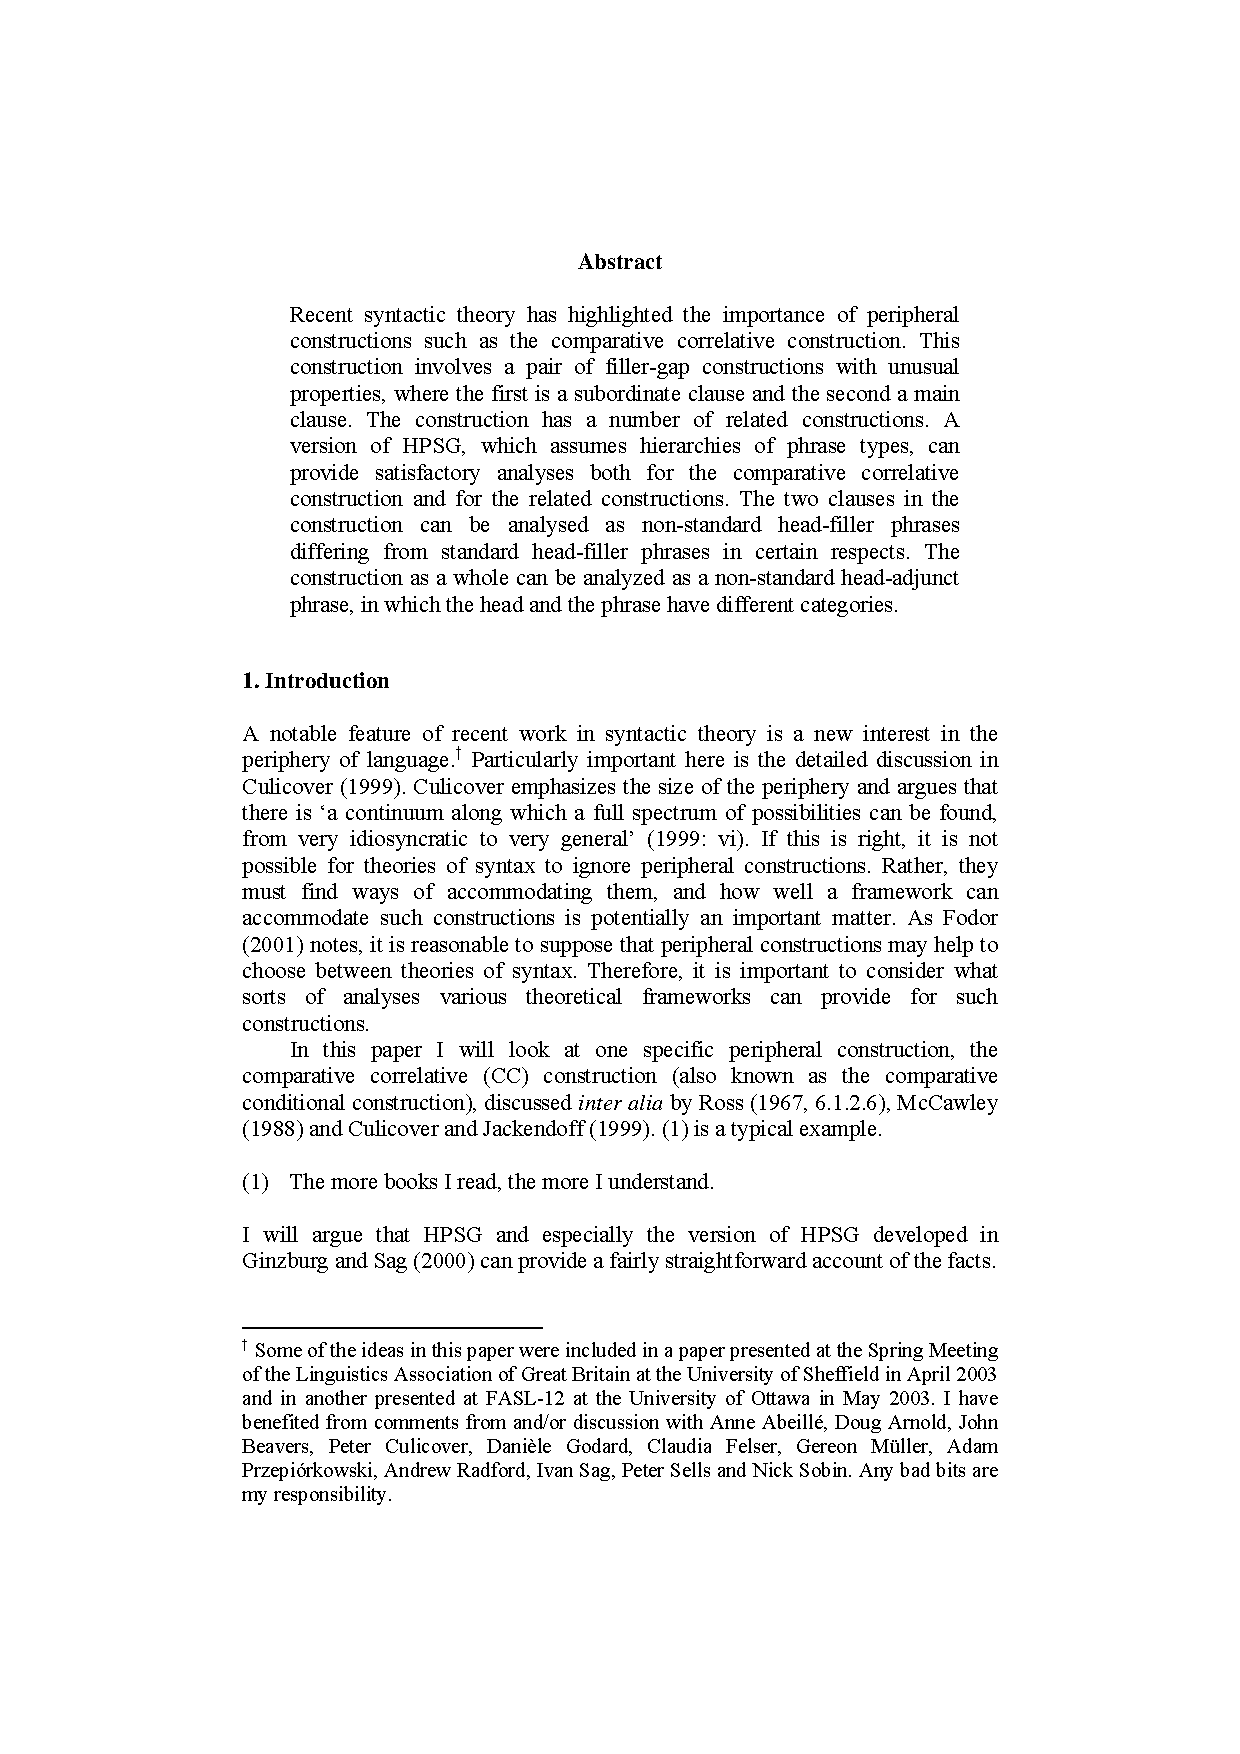
\includepdf[pages=-,pagecommand=\thispagestyle{plain}]{Includes/borsley.pdf}
        \setcounter{page}{93}
        \phantomsection
        \addcontentsline{toc}{section}{Michael W. Daniels, W. Detmar Meurers: GIDLP: A Grammar Format For Linearization-based HPSG}
\thispagestyle{empty}

\begin{center}
  {\huge\bfseries GIDLP: A Grammar Format For Linearization-based HPSG\par}

  \bigskip

~\\
\begingroup
\setlength{\leftskip}{0pt plus 1fill}
\setlength{\rightskip}{0pt plus 1fill}
\setlength{\parindent}{0pt}
\setlength{\parfillskip}{0pt}
  \formatauthor{Michael W. Daniels}{\begin{tabular}{@{}c@{}}Ohio State University\end{tabular}}
\formatauthor{W. Detmar Meurers}{\begin{tabular}{@{}c@{}}Ohio State University\end{tabular}}

\par\endgroup

  \vspace*{8ex}

  Proceedings of the 11th International Conference on\par Head-Driven Phrase Structure Grammar

  \bigskip

  Center for Computational Linguistics, Katholieke Universiteit Leuven

  \medskip

  Stefan Müller (Editor)

  \medskip

  2004

  \medskip

  CSLI Publications

  \medskip

  pages 93--111

  \medskip

  \url{http://csli-publications.stanford.edu/HPSG/2004}
\end{center}
\vfill

\noindent



\vfill
\noindent
% APA Style
Daniels, Michael W., \& Meurers, W. Detmar. 2004. GIDLP: A Grammar Format For Linearization-based HPSG. In Müller, Stefan (Ed.), \emph{{Proceedings of the 11th International Conference on Head-Driven Phrase Structure Grammar, Center for Computational Linguistics, Katholieke Universiteit Leuven}}, 93--111. Stanford,
CA: CSLI Publications. \hfill\href{http://creativecommons.org/licenses/by/4.0/}{\includegraphics[height=.75em]{Includes/ccby.eps}}

\newpage
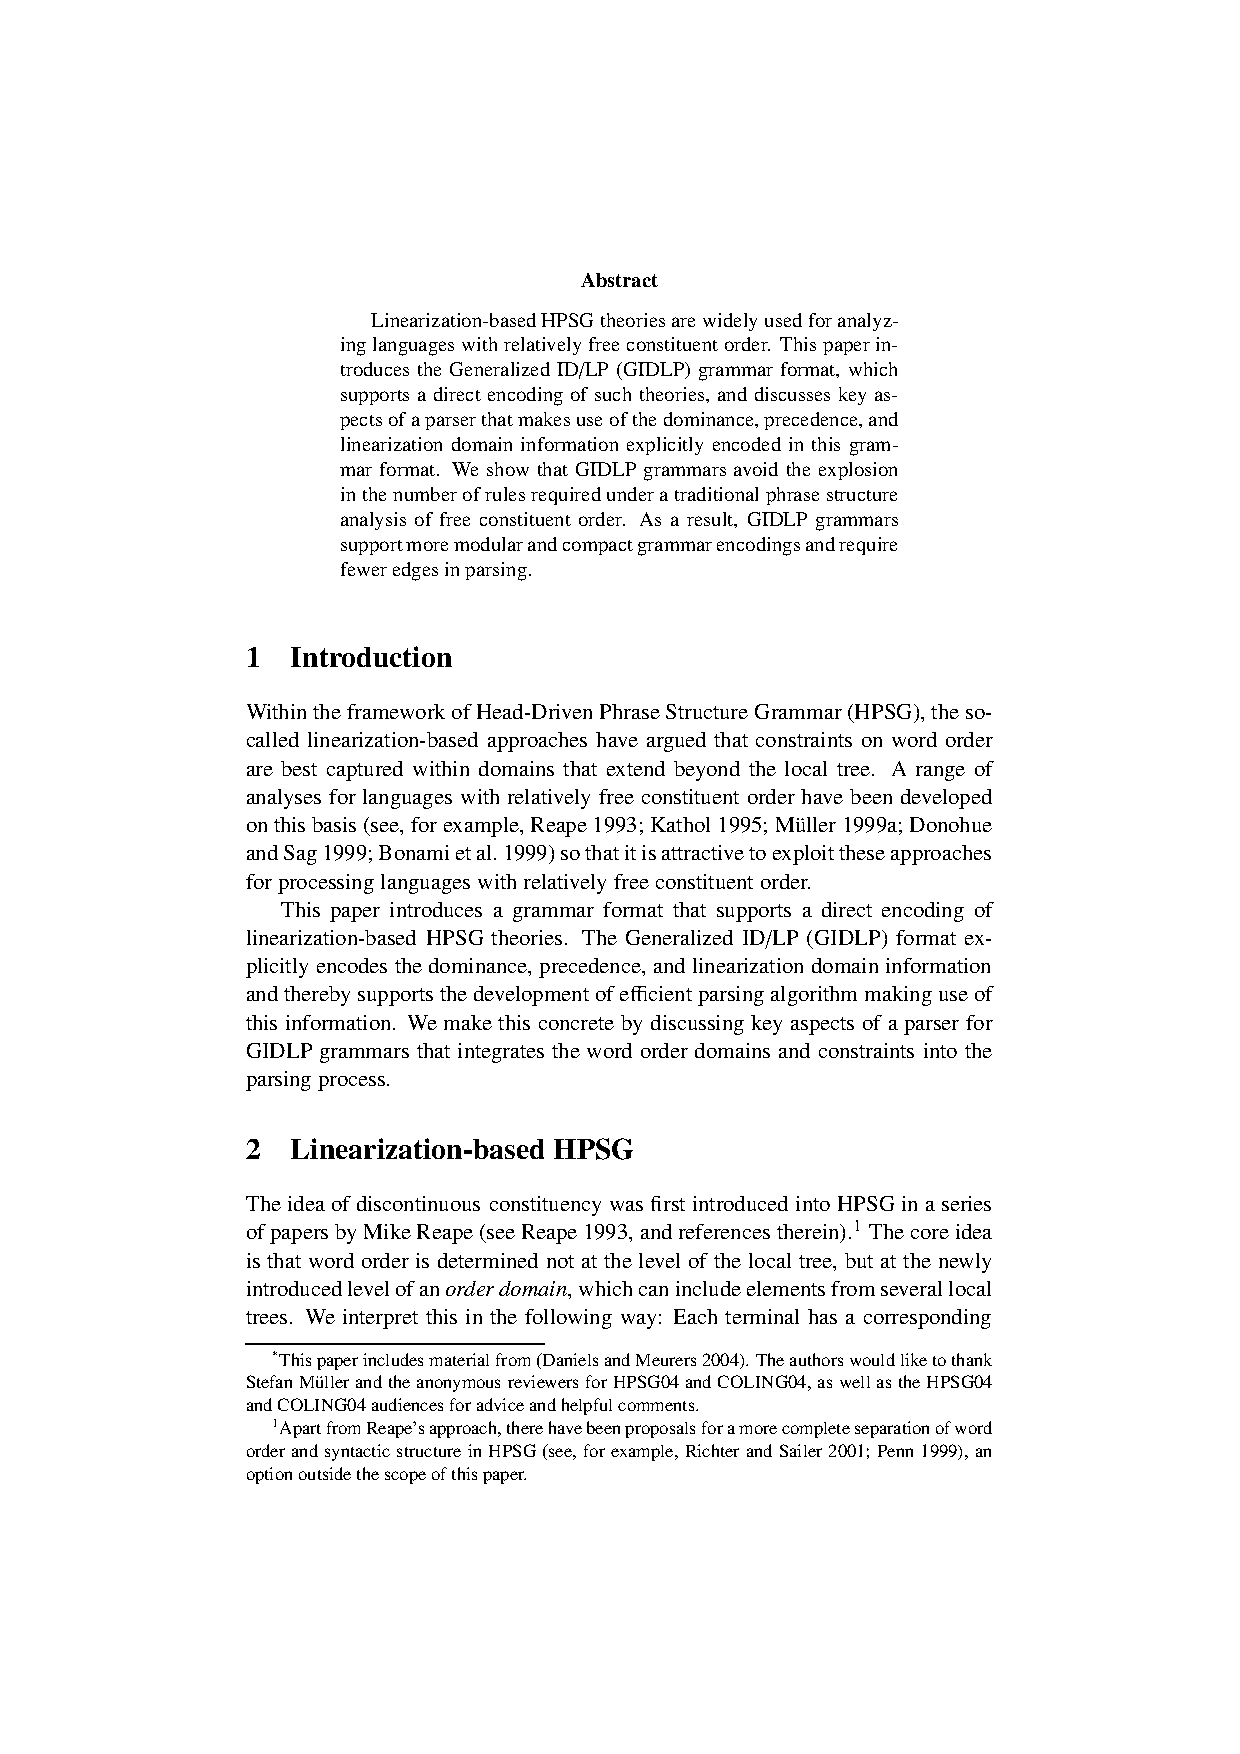
\includepdf[pages=-,pagecommand=\thispagestyle{plain}]{Includes/daniels-meurers.pdf}
        \setcounter{page}{112}
        \phantomsection
        \addcontentsline{toc}{section}{Henriette de Swart: A Typology of Negation in a Constraint-Based Framework of Syntax and Semantics}
\thispagestyle{empty}

\begin{center}
  {\huge\bfseries A Typology of Negation in a Constraint-Based Framework of Syntax and Semantics\par}

  \bigskip

~\\
\begingroup
\setlength{\leftskip}{0pt plus 1fill}
\setlength{\rightskip}{0pt plus 1fill}
\setlength{\parindent}{0pt}
\setlength{\parfillskip}{0pt}
  \formatauthor{Henriette de Swart}{\begin{tabular}{@{}c@{}}Universiteit Utrecht\end{tabular}}

\par\endgroup

  \vspace*{8ex}

  Proceedings of the 11th International Conference on\par Head-Driven Phrase Structure Grammar

  \bigskip

  Center for Computational Linguistics, Katholieke Universiteit Leuven

  \medskip

  Stefan Müller (Editor)

  \medskip

  2004

  \medskip

  CSLI Publications

  \medskip

  pages 112--118

  \medskip

  \url{http://csli-publications.stanford.edu/HPSG/2004}
\end{center}
\vfill

\noindent



\vfill
\noindent
% APA Style
de Swart, Henriette. 2004. A Typology of Negation in a Constraint-Based Framework of Syntax and Semantics. In Müller, Stefan (Ed.), \emph{{Proceedings of the 11th International Conference on Head-Driven Phrase Structure Grammar, Center for Computational Linguistics, Katholieke Universiteit Leuven}}, 112--118. Stanford,
CA: CSLI Publications. \hfill\href{http://creativecommons.org/licenses/by/4.0/}{\includegraphics[height=.75em]{Includes/ccby.eps}}

\newpage
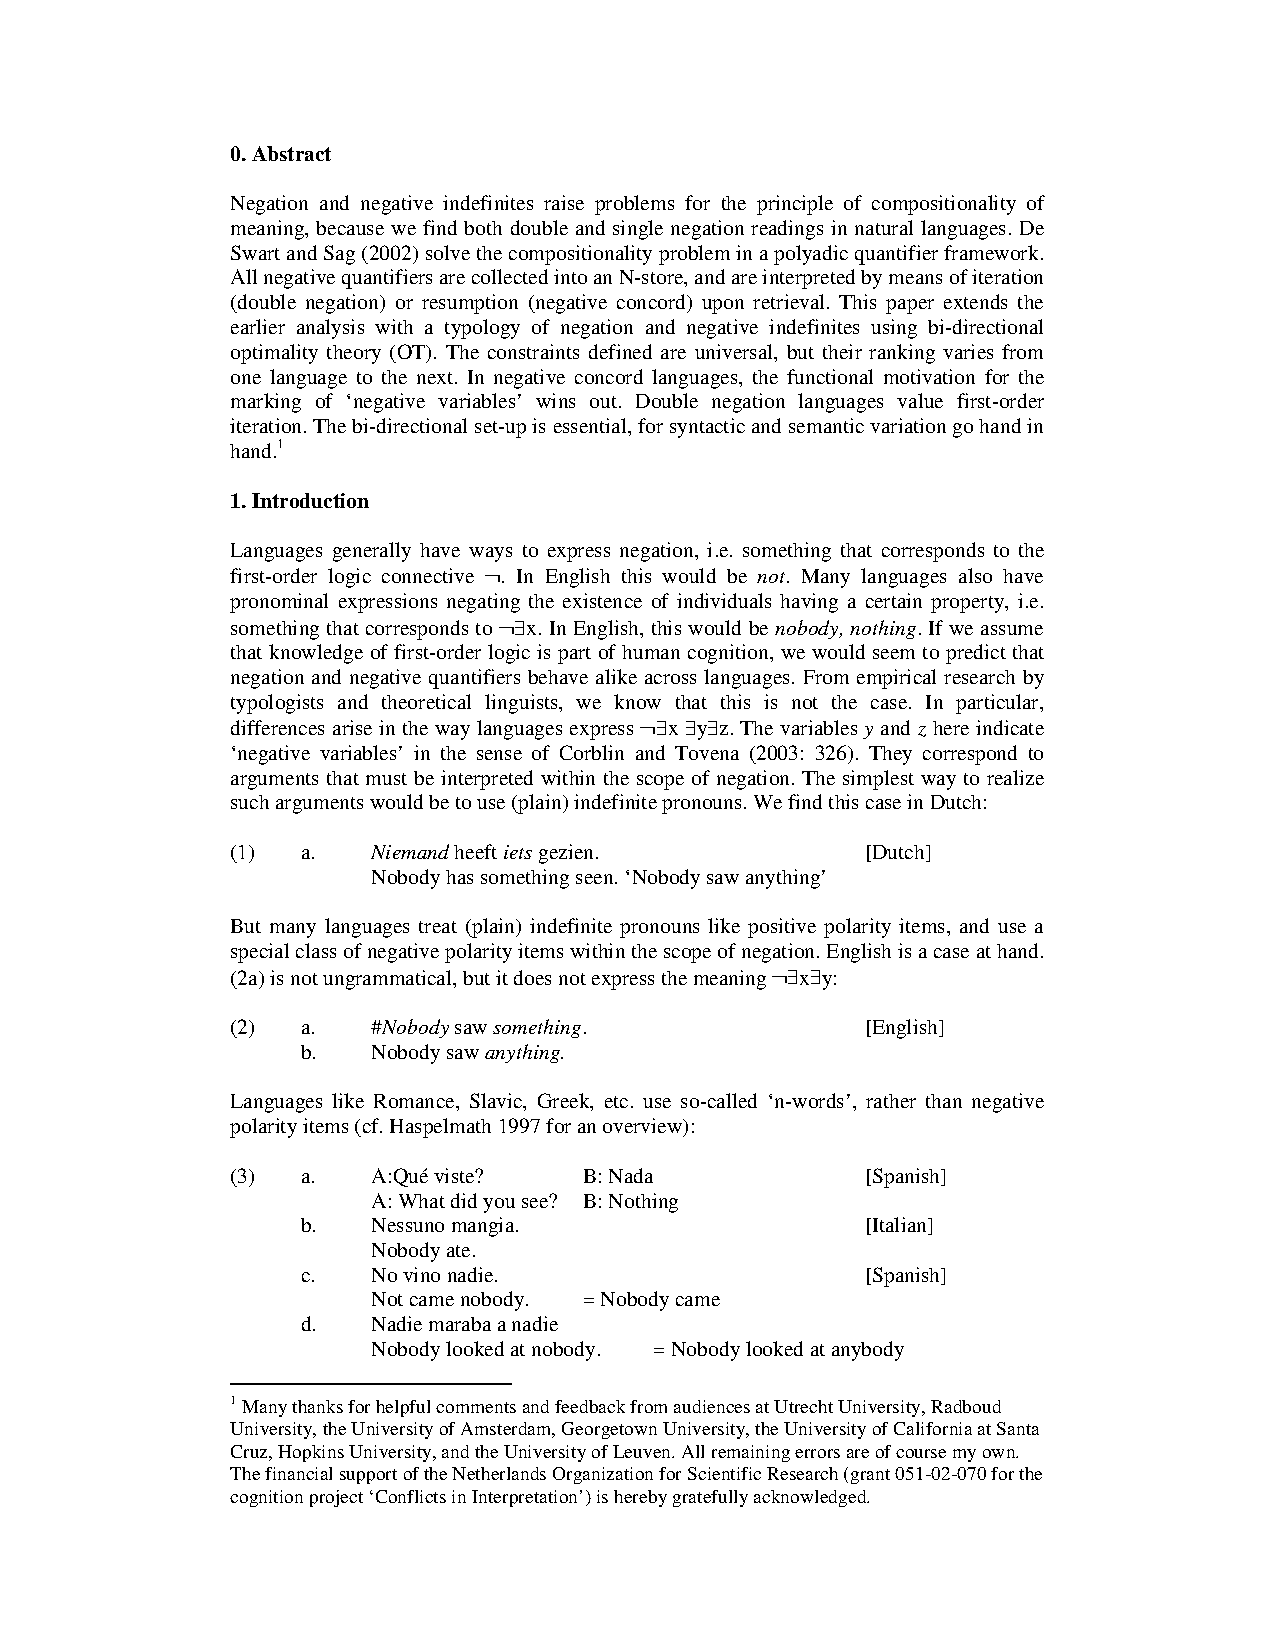
\includepdf[pages=-,pagecommand=\thispagestyle{plain}]{Includes/deswart.pdf}
        \setcounter{page}{119}
        \phantomsection
        \addcontentsline{toc}{section}{Markus Egg: Mismatches at the Syntax-Semantics Interface}
\thispagestyle{empty}

\begin{center}
  {\huge\bfseries Mismatches at the Syntax-Semantics Interface\par}

  \bigskip

~\\
\begingroup
\setlength{\leftskip}{0pt plus 1fill}
\setlength{\rightskip}{0pt plus 1fill}
\setlength{\parindent}{0pt}
\setlength{\parfillskip}{0pt}
  \formatauthor{Markus Egg}{\begin{tabular}{@{}c@{}}Universität Saarbrücken\end{tabular}}

\par\endgroup

  \vspace*{8ex}

  Proceedings of the 11th International Conference on\par Head-Driven Phrase Structure Grammar

  \bigskip

  Center for Computational Linguistics, Katholieke Universiteit Leuven

  \medskip

  Stefan Müller (Editor)

  \medskip

  2004

  \medskip

  CSLI Publications

  \medskip

  pages 119--139

  \medskip

  \url{http://csli-publications.stanford.edu/HPSG/2004}
\end{center}
\vfill

\noindent



\vfill
\noindent
% APA Style
Egg, Markus. 2004. Mismatches at the Syntax-Semantics Interface. In Müller, Stefan (Ed.), \emph{{Proceedings of the 11th International Conference on Head-Driven Phrase Structure Grammar, Center for Computational Linguistics, Katholieke Universiteit Leuven}}, 119--139. Stanford,
CA: CSLI Publications. \hfill\href{http://creativecommons.org/licenses/by/4.0/}{\includegraphics[height=.75em]{Includes/ccby.eps}}

\newpage
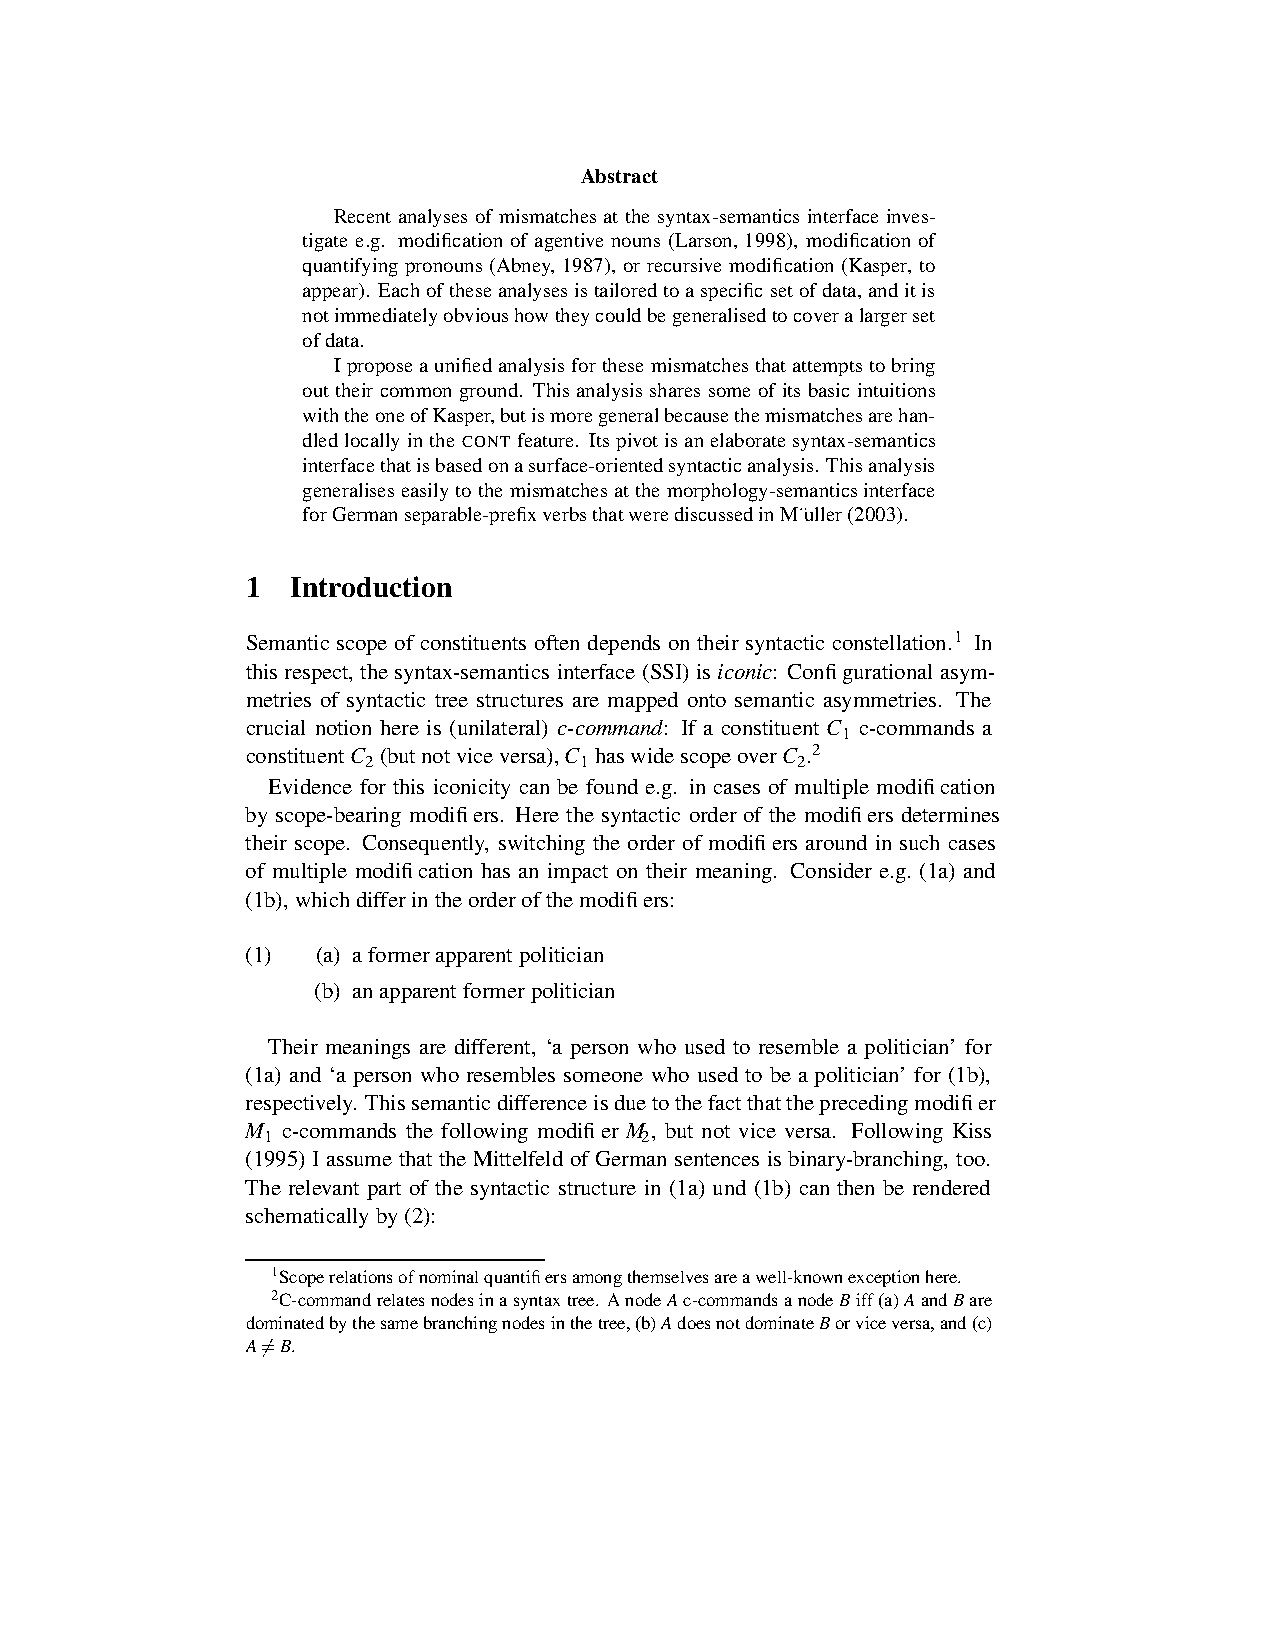
\includepdf[pages=-,pagecommand=\thispagestyle{plain}]{Includes/egg.pdf}
        \setcounter{page}{140}
        \phantomsection
        \addcontentsline{toc}{section}{Jean-Pierre Koenig, Anthony R. Davis: Raising Doubts about Russian Impersonals}
\thispagestyle{empty}

\begin{center}
  {\huge\bfseries Raising Doubts about Russian Impersonals\par}

  \bigskip

~\\
\begingroup
\setlength{\leftskip}{0pt plus 1fill}
\setlength{\rightskip}{0pt plus 1fill}
\setlength{\parindent}{0pt}
\setlength{\parfillskip}{0pt}
  \formatauthor{Jean-Pierre Koenig}{\begin{tabular}{@{}c@{}}University at Buffalo, The State University of New York\end{tabular}}
\formatauthor{Anthony R. Davis}{\begin{tabular}{@{}c@{}}StreamSage, Inc.\end{tabular}}

\par\endgroup

  \vspace*{8ex}

  Proceedings of the 11th International Conference on\par Head-Driven Phrase Structure Grammar

  \bigskip

  Center for Computational Linguistics, Katholieke Universiteit Leuven

  \medskip

  Stefan Müller (Editor)

  \medskip

  2004

  \medskip

  CSLI Publications

  \medskip

  pages 140--150

  \medskip

  \url{http://csli-publications.stanford.edu/HPSG/2004}
\end{center}
\vfill

\noindent



\vfill
\noindent
% APA Style
Koenig, Jean-Pierre, \& Davis, Anthony R. 2004. Raising Doubts about Russian Impersonals. In Müller, Stefan (Ed.), \emph{{Proceedings of the 11th International Conference on Head-Driven Phrase Structure Grammar, Center for Computational Linguistics, Katholieke Universiteit Leuven}}, 140--150. Stanford,
CA: CSLI Publications. \hfill\href{http://creativecommons.org/licenses/by/4.0/}{\includegraphics[height=.75em]{Includes/ccby.eps}}

\newpage
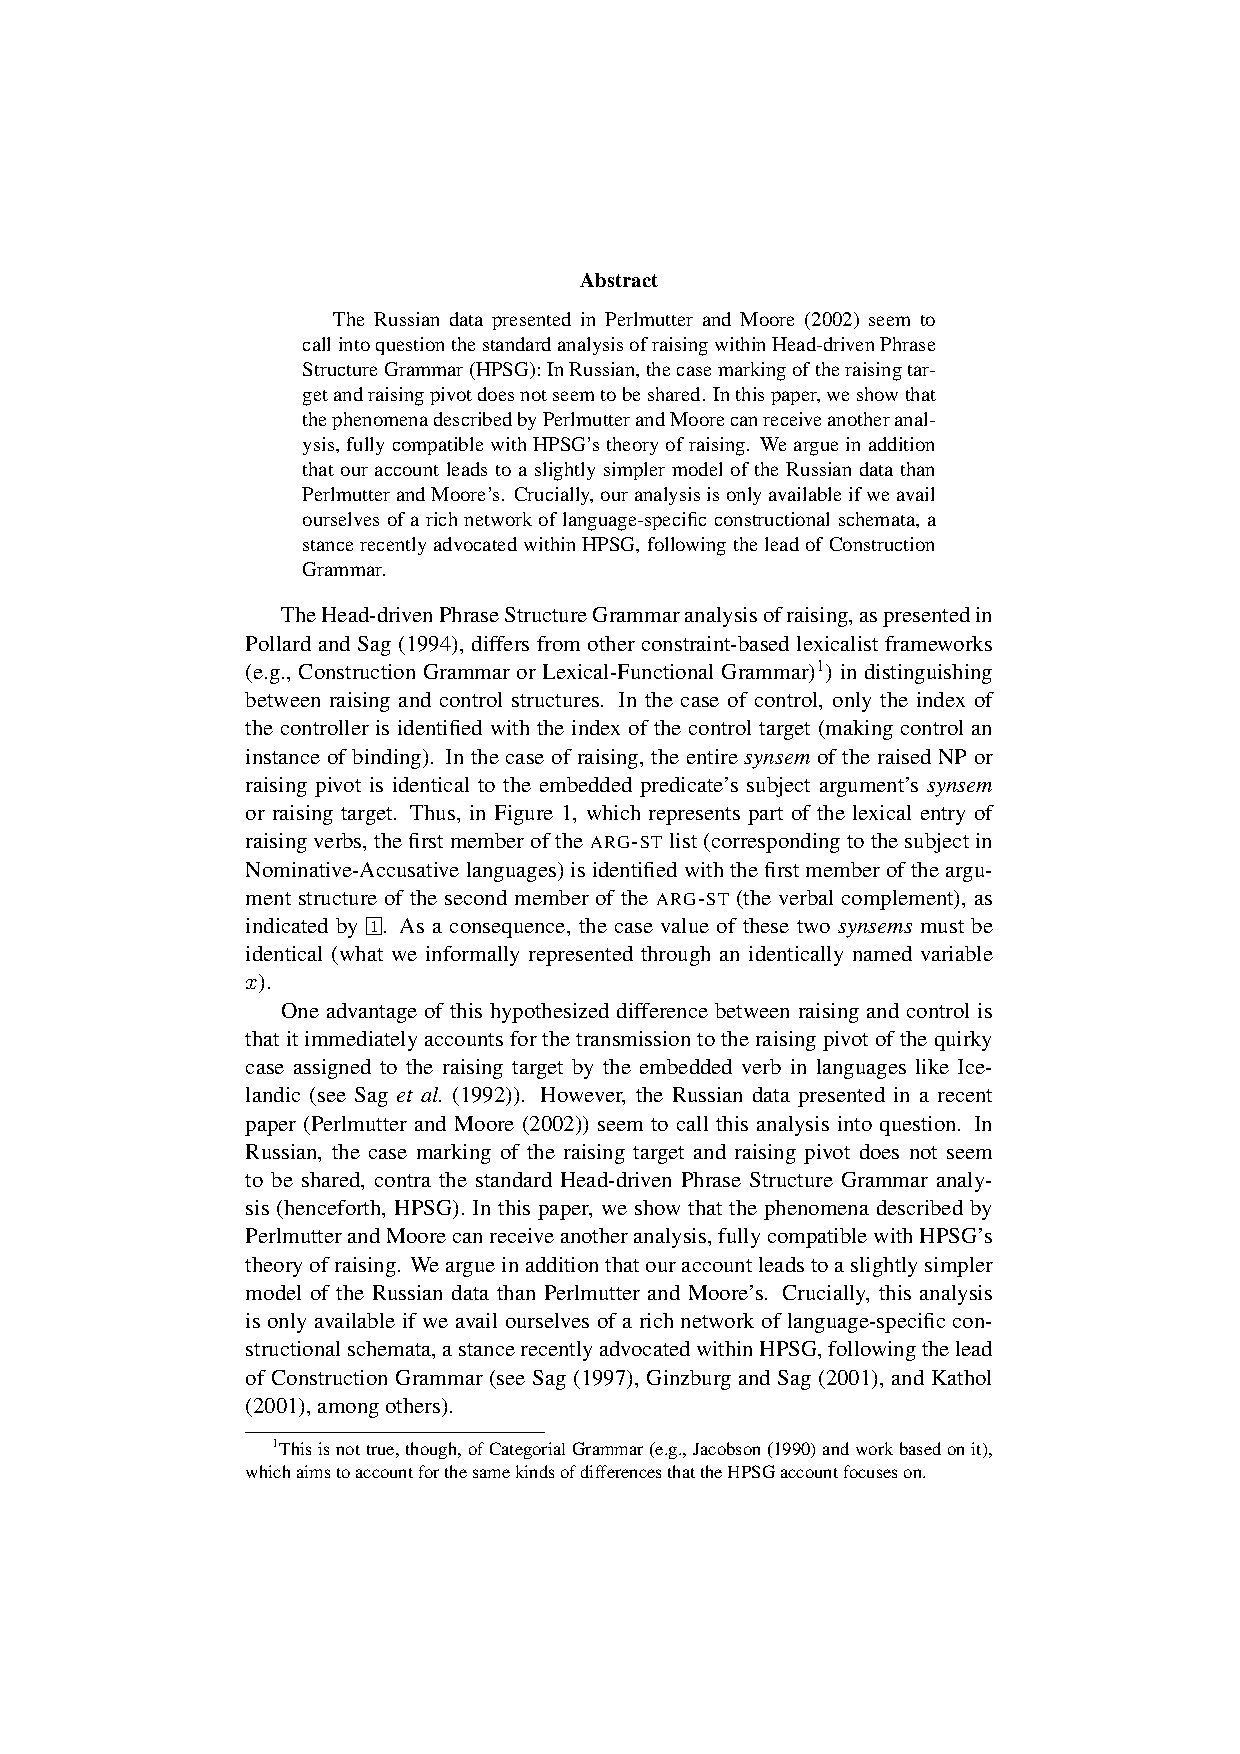
\includepdf[pages=-,pagecommand=\thispagestyle{plain}]{Includes/koenig-davis.pdf}
        \setcounter{page}{151}
        \phantomsection
        \addcontentsline{toc}{section}{Valia Kordoni: Between Shifts and Alternations: Ditransitive Constructions}
\thispagestyle{empty}

\begin{center}
  {\huge\bfseries Between Shifts and Alternations: Ditransitive Constructions\par}

  \bigskip

~\\
\begingroup
\setlength{\leftskip}{0pt plus 1fill}
\setlength{\rightskip}{0pt plus 1fill}
\setlength{\parindent}{0pt}
\setlength{\parfillskip}{0pt}
  \formatauthor{Valia Kordoni}{\begin{tabular}{@{}c@{}}Saarland University\end{tabular}}

\par\endgroup

  \vspace*{8ex}

  Proceedings of the 11th International Conference on\par Head-Driven Phrase Structure Grammar

  \bigskip

  Center for Computational Linguistics, Katholieke Universiteit Leuven

  \medskip

  Stefan Müller (Editor)

  \medskip

  2004

  \medskip

  CSLI Publications

  \medskip

  pages 151--167

  \medskip

  \url{http://csli-publications.stanford.edu/HPSG/2004}
\end{center}
\vfill

\noindent



\vfill
\noindent
% APA Style
Kordoni, Valia. 2004. Between Shifts and Alternations: Ditransitive Constructions. In Müller, Stefan (Ed.), \emph{{Proceedings of the 11th International Conference on Head-Driven Phrase Structure Grammar, Center for Computational Linguistics, Katholieke Universiteit Leuven}}, 151--167. Stanford,
CA: CSLI Publications. \hfill\href{http://creativecommons.org/licenses/by/4.0/}{\includegraphics[height=.75em]{Includes/ccby.eps}}

\newpage
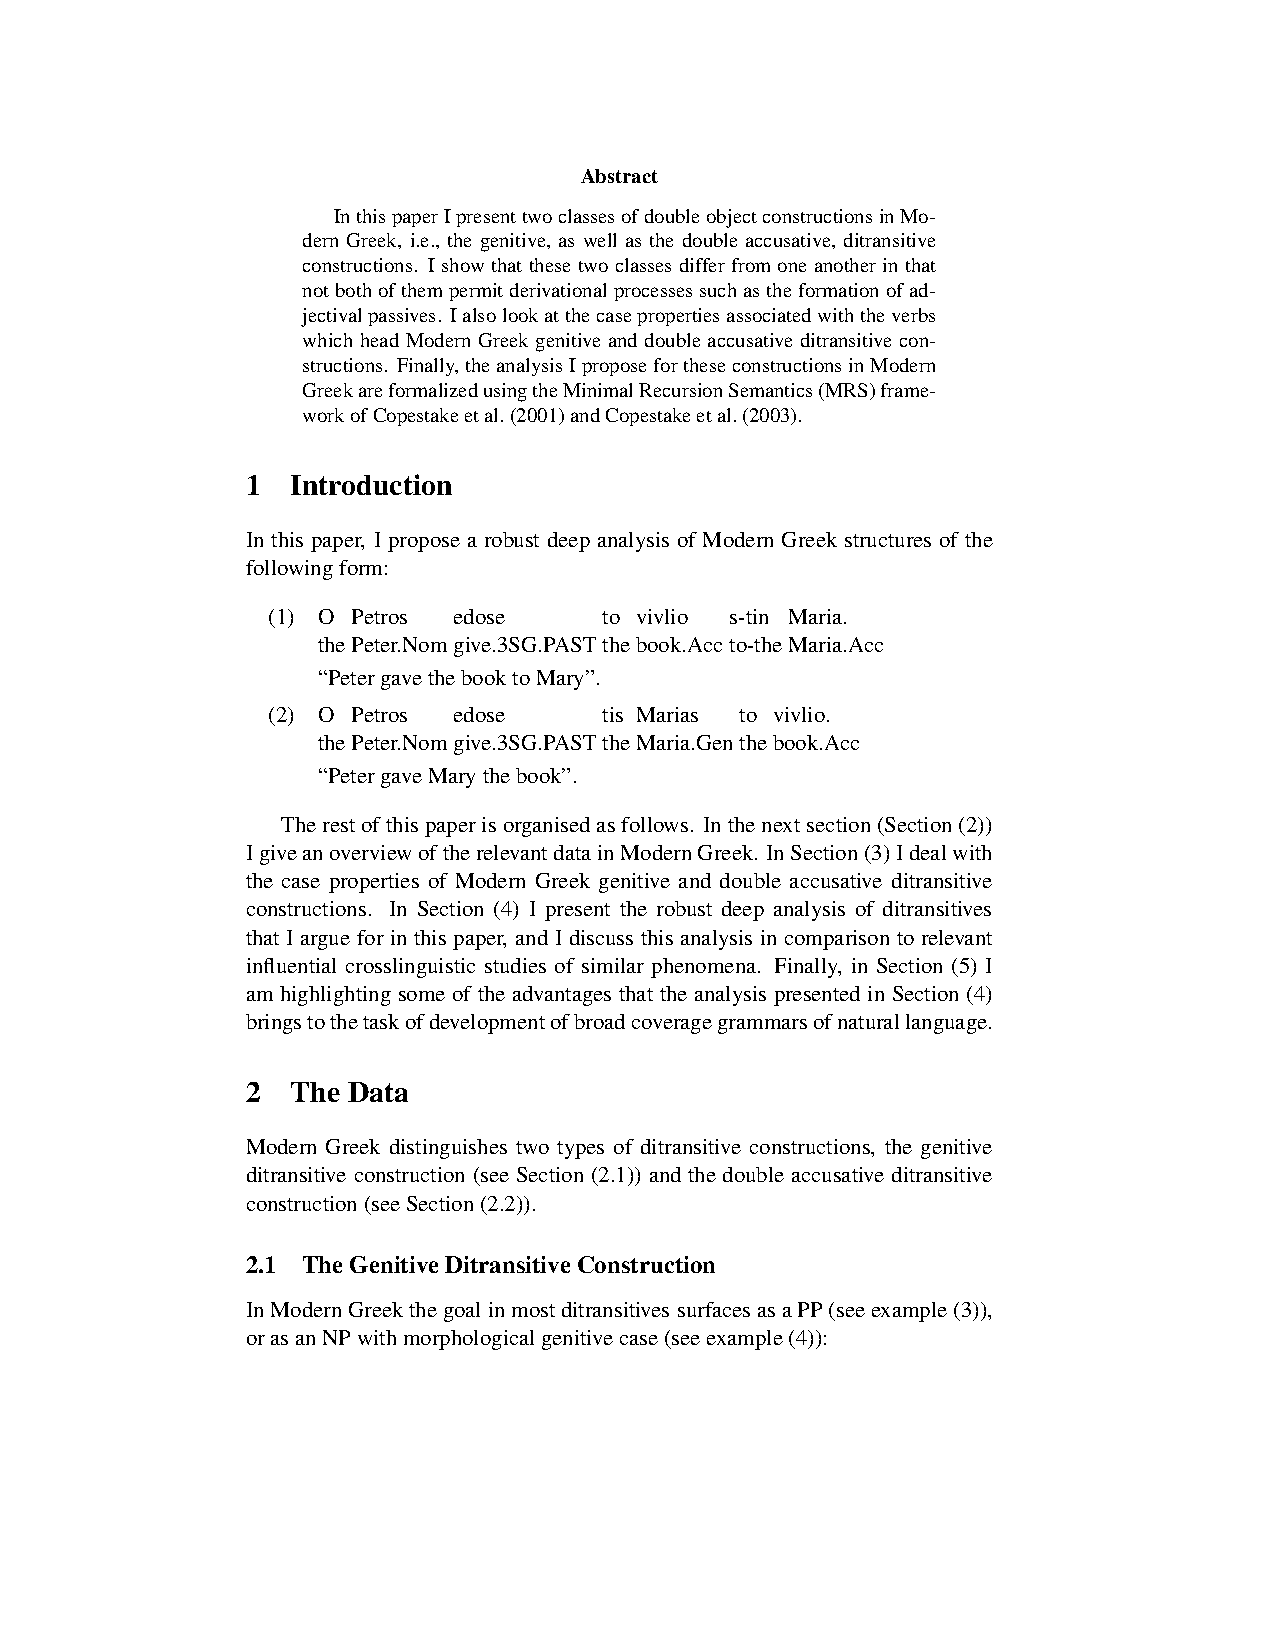
\includepdf[pages=-,pagecommand=\thispagestyle{plain}]{Includes/kordoni.pdf}
        \setcounter{page}{168}
        \phantomsection
        \addcontentsline{toc}{section}{Takafumi Maekawa: Constituency, Word Order and Focus Projection}
\thispagestyle{empty}

\begin{center}
  {\huge\bfseries Constituency, Word Order and Focus Projection\par}

  \bigskip

~\\
\begingroup
\setlength{\leftskip}{0pt plus 1fill}
\setlength{\rightskip}{0pt plus 1fill}
\setlength{\parindent}{0pt}
\setlength{\parfillskip}{0pt}
  \formatauthor{Takafumi Maekawa}{\begin{tabular}{@{}c@{}}University of Essex\end{tabular}}

\par\endgroup

  \vspace*{8ex}

  Proceedings of the 11th International Conference on\par Head-Driven Phrase Structure Grammar

  \bigskip

  Center for Computational Linguistics, Katholieke Universiteit Leuven

  \medskip

  Stefan Müller (Editor)

  \medskip

  2004

  \medskip

  CSLI Publications

  \medskip

  pages 168--188

  \medskip

  \url{http://csli-publications.stanford.edu/HPSG/2004}
\end{center}
\vfill

\noindent



\vfill
\noindent
% APA Style
Maekawa, Takafumi. 2004. Constituency, Word Order and Focus Projection. In Müller, Stefan (Ed.), \emph{{Proceedings of the 11th International Conference on Head-Driven Phrase Structure Grammar, Center for Computational Linguistics, Katholieke Universiteit Leuven}}, 168--188. Stanford,
CA: CSLI Publications. \hfill\href{http://creativecommons.org/licenses/by/4.0/}{\includegraphics[height=.75em]{Includes/ccby.eps}}

\newpage
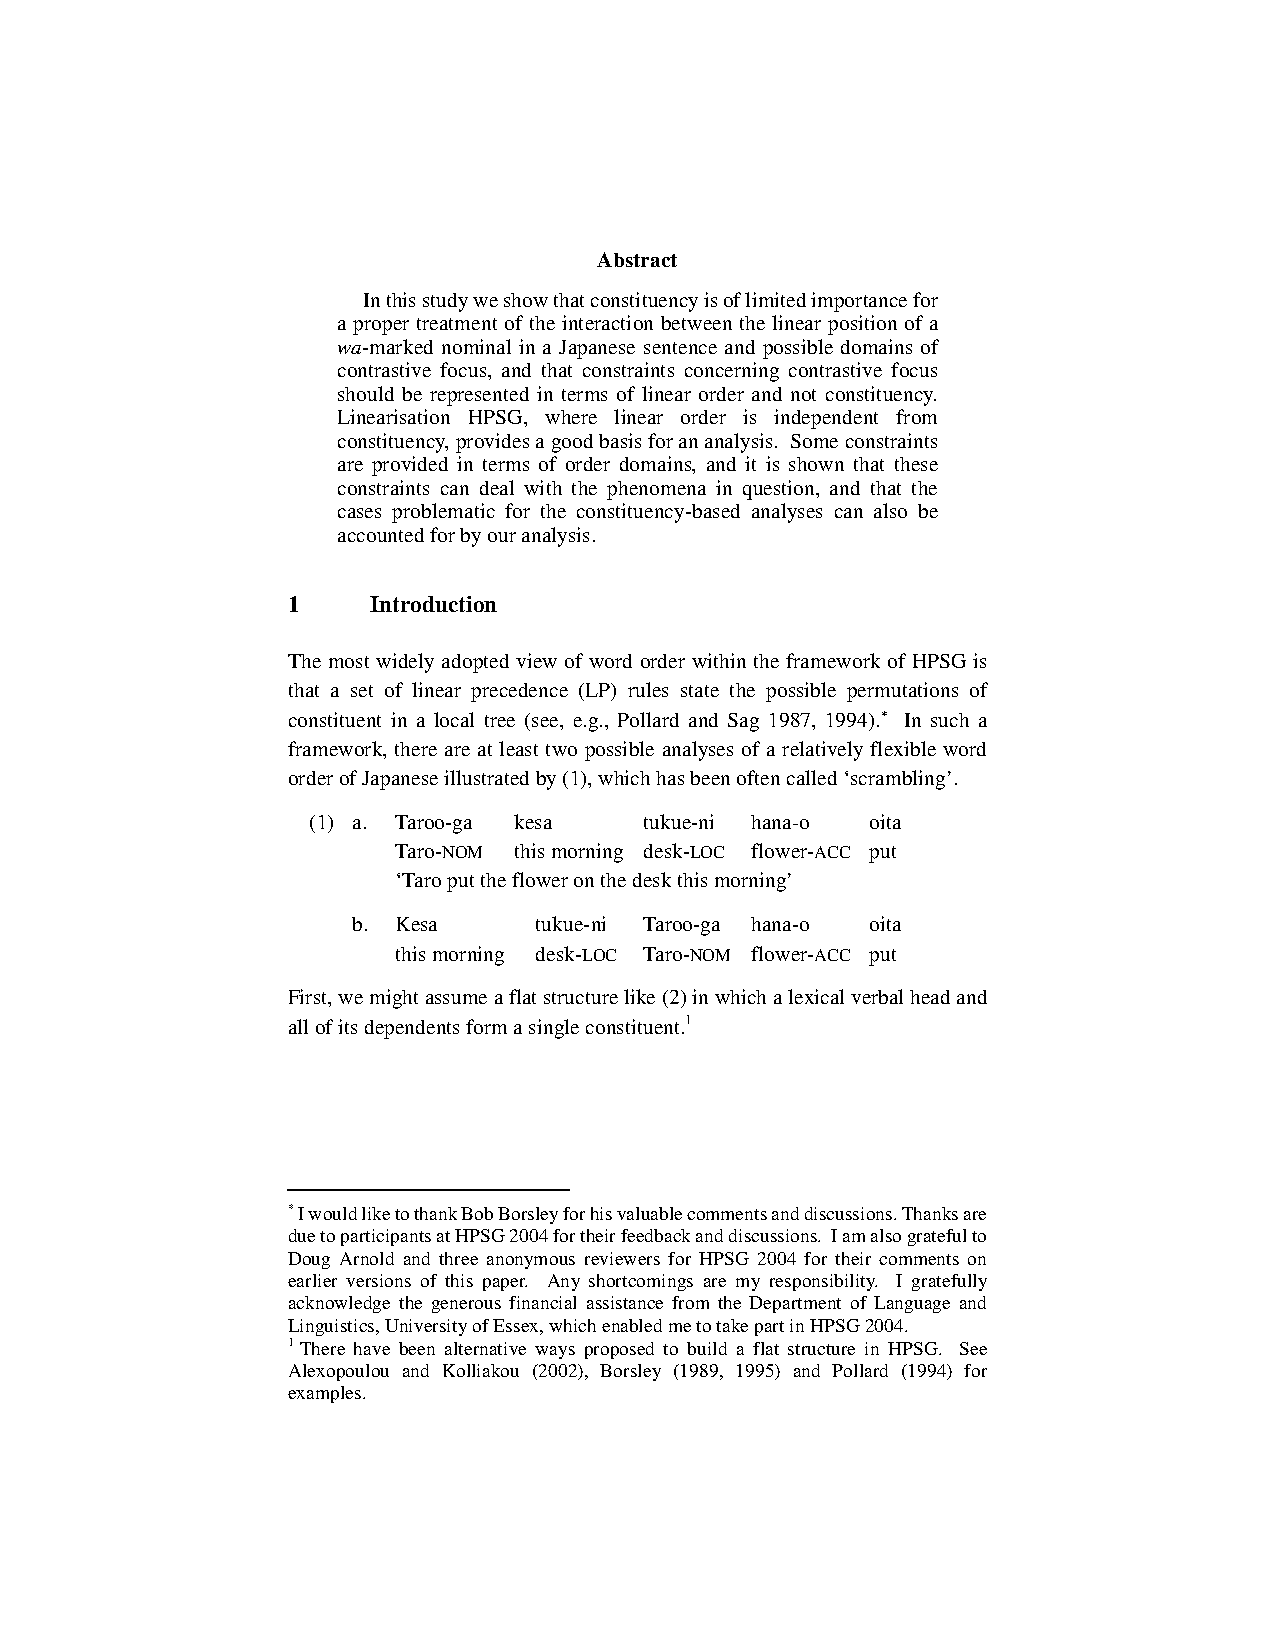
\includepdf[pages=-,pagecommand=\thispagestyle{plain}]{Includes/maekawa.pdf}
        \setcounter{page}{189}
        \phantomsection
        \addcontentsline{toc}{section}{Ian Marshall, Eva Safar: Sign Language Generation in an ALE HPSG}
\thispagestyle{empty}

\begin{center}
  {\huge\bfseries Sign Language Generation in an ALE HPSG\par}

  \bigskip

~\\
\begingroup
\setlength{\leftskip}{0pt plus 1fill}
\setlength{\rightskip}{0pt plus 1fill}
\setlength{\parindent}{0pt}
\setlength{\parfillskip}{0pt}
  \formatauthor{Ian Marshall}{\begin{tabular}{@{}c@{}}University of East Anglia\end{tabular}}
\formatauthor{Eva Safar}{\begin{tabular}{@{}c@{}}University of East Anglia\end{tabular}}

\par\endgroup

  \vspace*{8ex}

  Proceedings of the 11th International Conference on\par Head-Driven Phrase Structure Grammar

  \bigskip

  Center for Computational Linguistics, Katholieke Universiteit Leuven

  \medskip

  Stefan Müller (Editor)

  \medskip

  2004

  \medskip

  CSLI Publications

  \medskip

  pages 189--201

  \medskip

  \url{http://csli-publications.stanford.edu/HPSG/2004}
\end{center}
\vfill

\noindent



\vfill
\noindent
% APA Style
Marshall, Ian, \& Safar,  Eva. 2004. Sign Language Generation in an ALE HPSG. In Müller, Stefan (Ed.), \emph{{Proceedings of the 11th International Conference on Head-Driven Phrase Structure Grammar, Center for Computational Linguistics, Katholieke Universiteit Leuven}}, 189--201. Stanford,
CA: CSLI Publications. \hfill\href{http://creativecommons.org/licenses/by/4.0/}{\includegraphics[height=.75em]{Includes/ccby.eps}}

\newpage
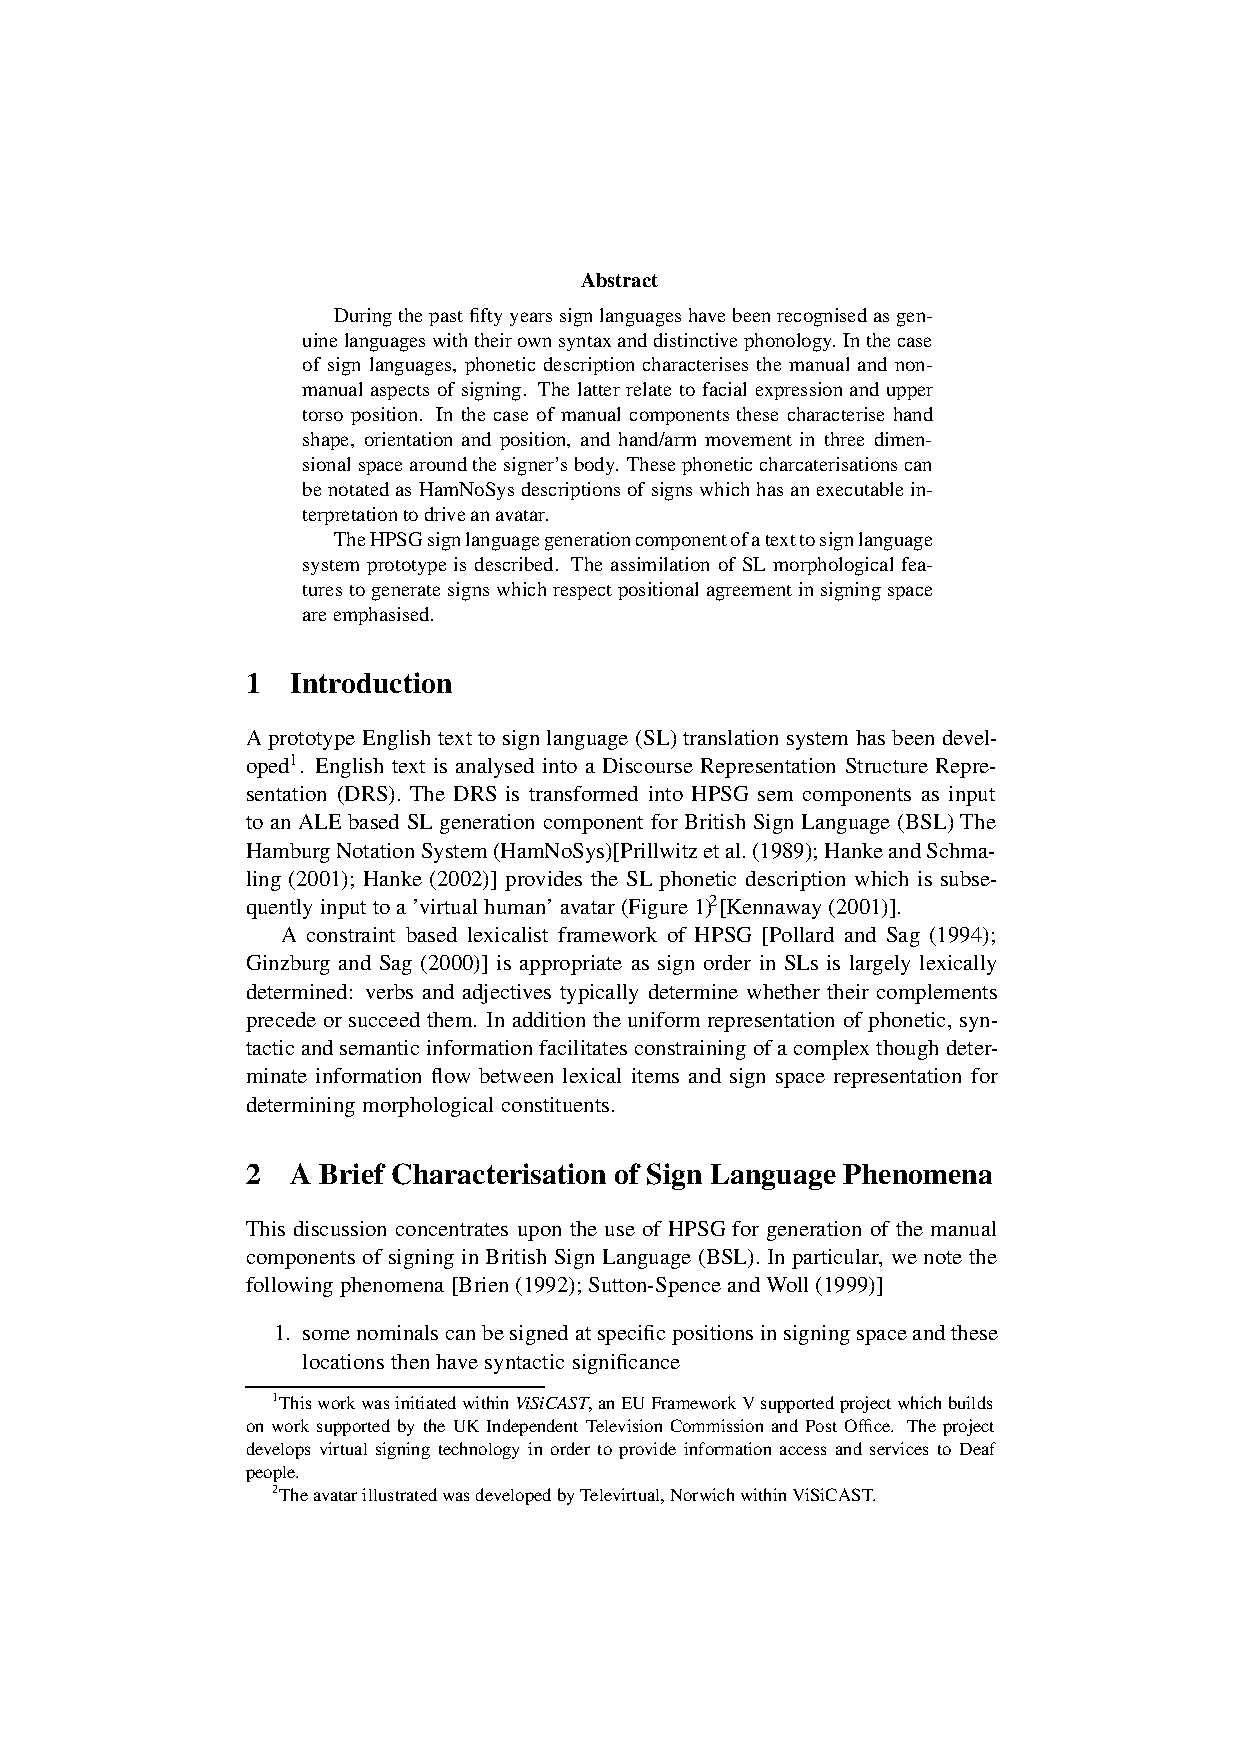
\includepdf[pages=-,pagecommand=\thispagestyle{plain}]{Includes/marshall-safar.pdf}
        \setcounter{page}{202}
        \phantomsection
        \addcontentsline{toc}{section}{Stefan M{\"u}ller: An Analysis of Depictive Secondary Predicates in German without Discontinuous Constituents}
\thispagestyle{empty}

\begin{center}
  {\huge\bfseries An Analysis of Depictive Secondary Predicates in German without Discontinuous Constituents\par}

  \bigskip

~\\
\begingroup
\setlength{\leftskip}{0pt plus 1fill}
\setlength{\rightskip}{0pt plus 1fill}
\setlength{\parindent}{0pt}
\setlength{\parfillskip}{0pt}
  \formatauthor{Stefan Müller}{\begin{tabular}{@{}c@{}}Universität Bremen\end{tabular}}

\par\endgroup

  \vspace*{8ex}

  Proceedings of the 11th International Conference on\par Head-Driven Phrase Structure Grammar

  \bigskip

  Center for Computational Linguistics, Katholieke Universiteit Leuven

  \medskip

  Stefan Müller (Editor)

  \medskip

  2004

  \medskip

  CSLI Publications

  \medskip

  pages 202--222

  \medskip

  \url{http://csli-publications.stanford.edu/HPSG/2004}
\end{center}
\vfill

\noindent



\vfill
\noindent
% APA Style
Müller, Stefan. 2004. An Analysis of Depictive Secondary Predicates in German without Discontinuous Constituents. In Müller, Stefan (Ed.), \emph{{Proceedings of the 11th International Conference on Head-Driven Phrase Structure Grammar, Center for Computational Linguistics, Katholieke Universiteit Leuven}}, 202--222. Stanford,
CA: CSLI Publications. \hfill\href{http://creativecommons.org/licenses/by/4.0/}{\includegraphics[height=.75em]{Includes/ccby.eps}}

\newpage
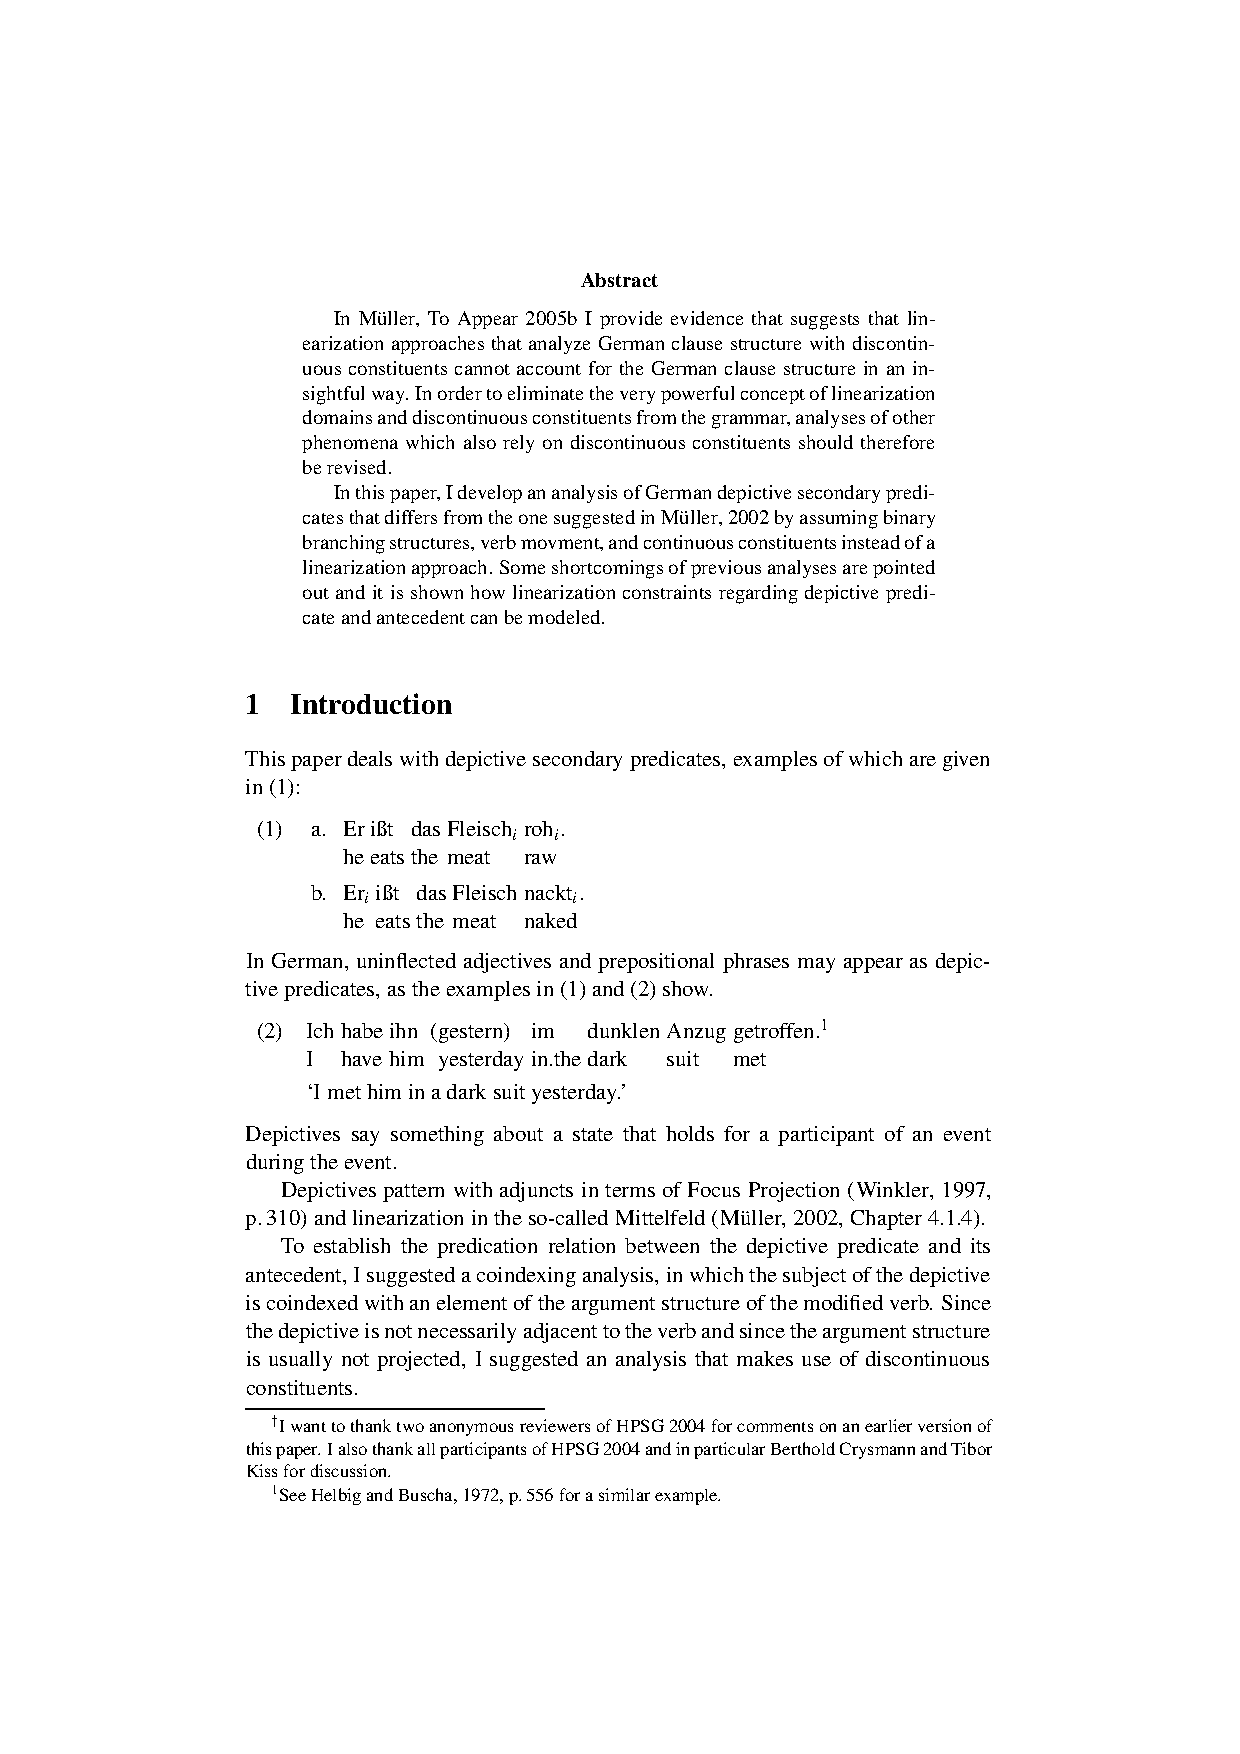
\includepdf[pages=-,pagecommand=\thispagestyle{plain}]{Includes/mueller.pdf}
        \setcounter{page}{223}
        \phantomsection
        \addcontentsline{toc}{section}{Manfred Sailer: Propositional Relative Clauses in German}
\thispagestyle{empty}

\begin{center}
  {\huge\bfseries Propositional Relative Clauses in German\par}

  \bigskip

~\\
\begingroup
\setlength{\leftskip}{0pt plus 1fill}
\setlength{\rightskip}{0pt plus 1fill}
\setlength{\parindent}{0pt}
\setlength{\parfillskip}{0pt}
  \formatauthor{Manfred Sailer}{\begin{tabular}{@{}c@{}}Universität Göttingen\end{tabular}}

\par\endgroup

  \vspace*{8ex}

  Proceedings of the 11th International Conference on\par Head-Driven Phrase Structure Grammar

  \bigskip

  Center for Computational Linguistics, Katholieke Universiteit Leuven

  \medskip

  Stefan Müller (Editor)

  \medskip

  2004

  \medskip

  CSLI Publications

  \medskip

  pages 223--243

  \medskip

  \url{http://csli-publications.stanford.edu/HPSG/2004}
\end{center}
\vfill

\noindent



\vfill
\noindent
% APA Style
Sailer, Manfred. 2004. Propositional Relative Clauses in German. In Müller, Stefan (Ed.), \emph{{Proceedings of the 11th International Conference on Head-Driven Phrase Structure Grammar, Center for Computational Linguistics, Katholieke Universiteit Leuven}}, 223--243. Stanford,
CA: CSLI Publications. \hfill\href{http://creativecommons.org/licenses/by/4.0/}{\includegraphics[height=.75em]{Includes/ccby.eps}}

\newpage
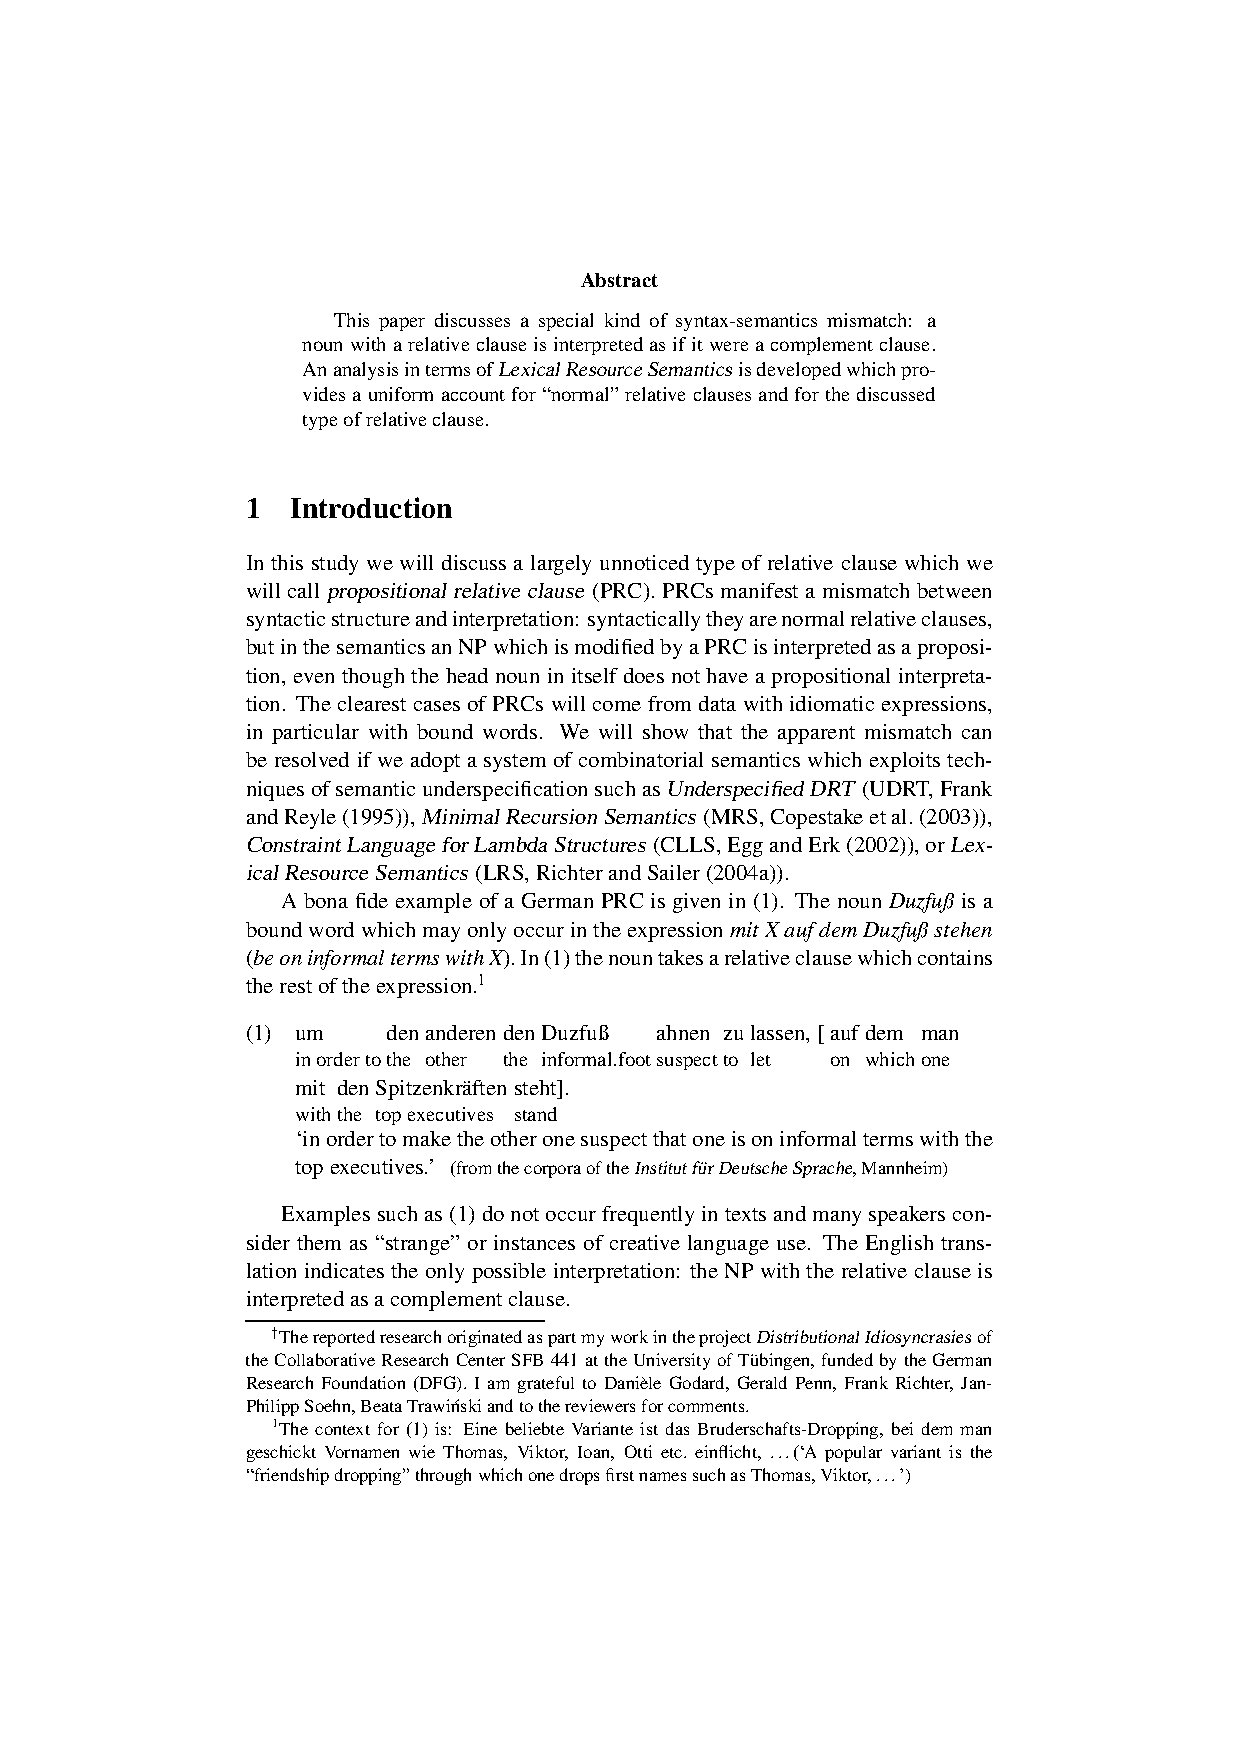
\includepdf[pages=-,pagecommand=\thispagestyle{plain}]{Includes/sailer.pdf}
        \setcounter{page}{244}
        \phantomsection
        \addcontentsline{toc}{section}{Melanie Siegel, Emily M. Bender: Head-Initial Constructions in Japanese}
\thispagestyle{empty}

\begin{center}
  {\huge\bfseries Head-Initial Constructions in Japanese\par}

  \bigskip

~\\
\begingroup
\setlength{\leftskip}{0pt plus 1fill}
\setlength{\rightskip}{0pt plus 1fill}
\setlength{\parindent}{0pt}
\setlength{\parfillskip}{0pt}
  \formatauthor{Melanie Siegel}{\begin{tabular}{@{}c@{}}University of Saarbrücken\end{tabular}}
\formatauthor{Emily M. Bender}{\begin{tabular}{@{}c@{}}University of Washington\end{tabular}}

\par\endgroup

  \vspace*{8ex}

  Proceedings of the 11th International Conference on\par Head-Driven Phrase Structure Grammar

  \bigskip

  Center for Computational Linguistics, Katholieke Universiteit Leuven

  \medskip

  Stefan Müller (Editor)

  \medskip

  2004

  \medskip

  CSLI Publications

  \medskip

  pages 244--260

  \medskip

  \url{http://csli-publications.stanford.edu/HPSG/2004}
\end{center}
\vfill

\noindent



\vfill
\noindent
% APA Style
Siegel, Melanie, \& Bender, Emily M. 2004. Head-Initial Constructions in Japanese. In Müller, Stefan (Ed.), \emph{{Proceedings of the 11th International Conference on Head-Driven Phrase Structure Grammar, Center for Computational Linguistics, Katholieke Universiteit Leuven}}, 244--260. Stanford,
CA: CSLI Publications. \hfill\href{http://creativecommons.org/licenses/by/4.0/}{\includegraphics[height=.75em]{Includes/ccby.eps}}

\newpage
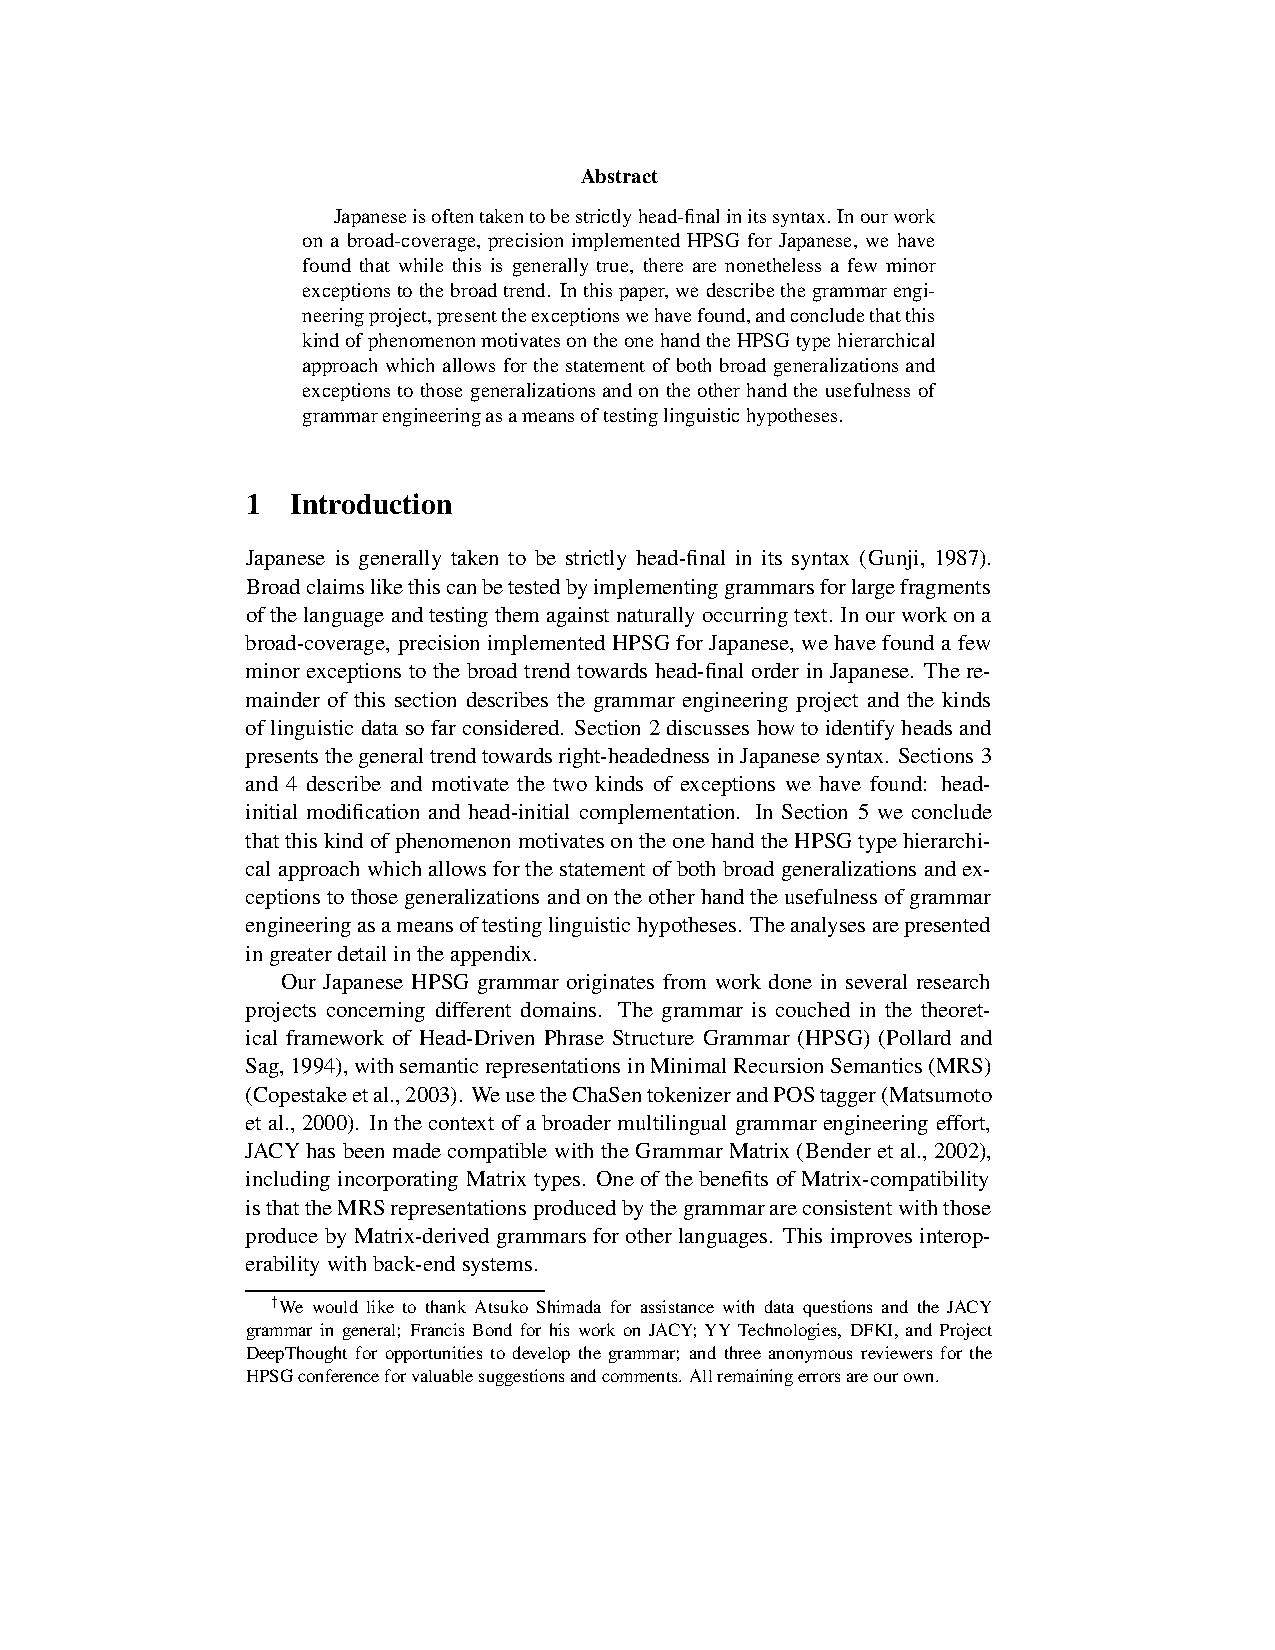
\includepdf[pages=-,pagecommand=\thispagestyle{plain}]{Includes/siegel-bender.pdf}
        \setcounter{page}{261}
        \phantomsection
        \addcontentsline{toc}{section}{Jan-Philipp Soehn: License to Coll: How to Bind Bound Words and Readings to their Contexts}
\thispagestyle{empty}

\begin{center}
  {\huge\bfseries License to Coll: How to Bind Bound Words and Readings to their Contexts\par}

  \bigskip

~\\
\begingroup
\setlength{\leftskip}{0pt plus 1fill}
\setlength{\rightskip}{0pt plus 1fill}
\setlength{\parindent}{0pt}
\setlength{\parfillskip}{0pt}
  \formatauthor{Jan-Philipp Soehn}{\begin{tabular}{@{}c@{}}University of Jena\end{tabular}}

\par\endgroup

  \vspace*{8ex}

  Proceedings of the 11th International Conference on\par Head-Driven Phrase Structure Grammar

  \bigskip

  Center for Computational Linguistics, Katholieke Universiteit Leuven

  \medskip

  Stefan Müller (Editor)

  \medskip

  2004

  \medskip

  CSLI Publications

  \medskip

  pages 261--273

  \medskip

  \url{http://csli-publications.stanford.edu/HPSG/2004}
\end{center}
\vfill

\noindent



\vfill
\noindent
% APA Style
Soehn, Jan-Philipp. 2004. License to Coll: How to Bind Bound Words and Readings to their Contexts. In Müller, Stefan (Ed.), \emph{{Proceedings of the 11th International Conference on Head-Driven Phrase Structure Grammar, Center for Computational Linguistics, Katholieke Universiteit Leuven}}, 261--273. Stanford,
CA: CSLI Publications. \hfill\href{http://creativecommons.org/licenses/by/4.0/}{\includegraphics[height=.75em]{Includes/ccby.eps}}

\newpage
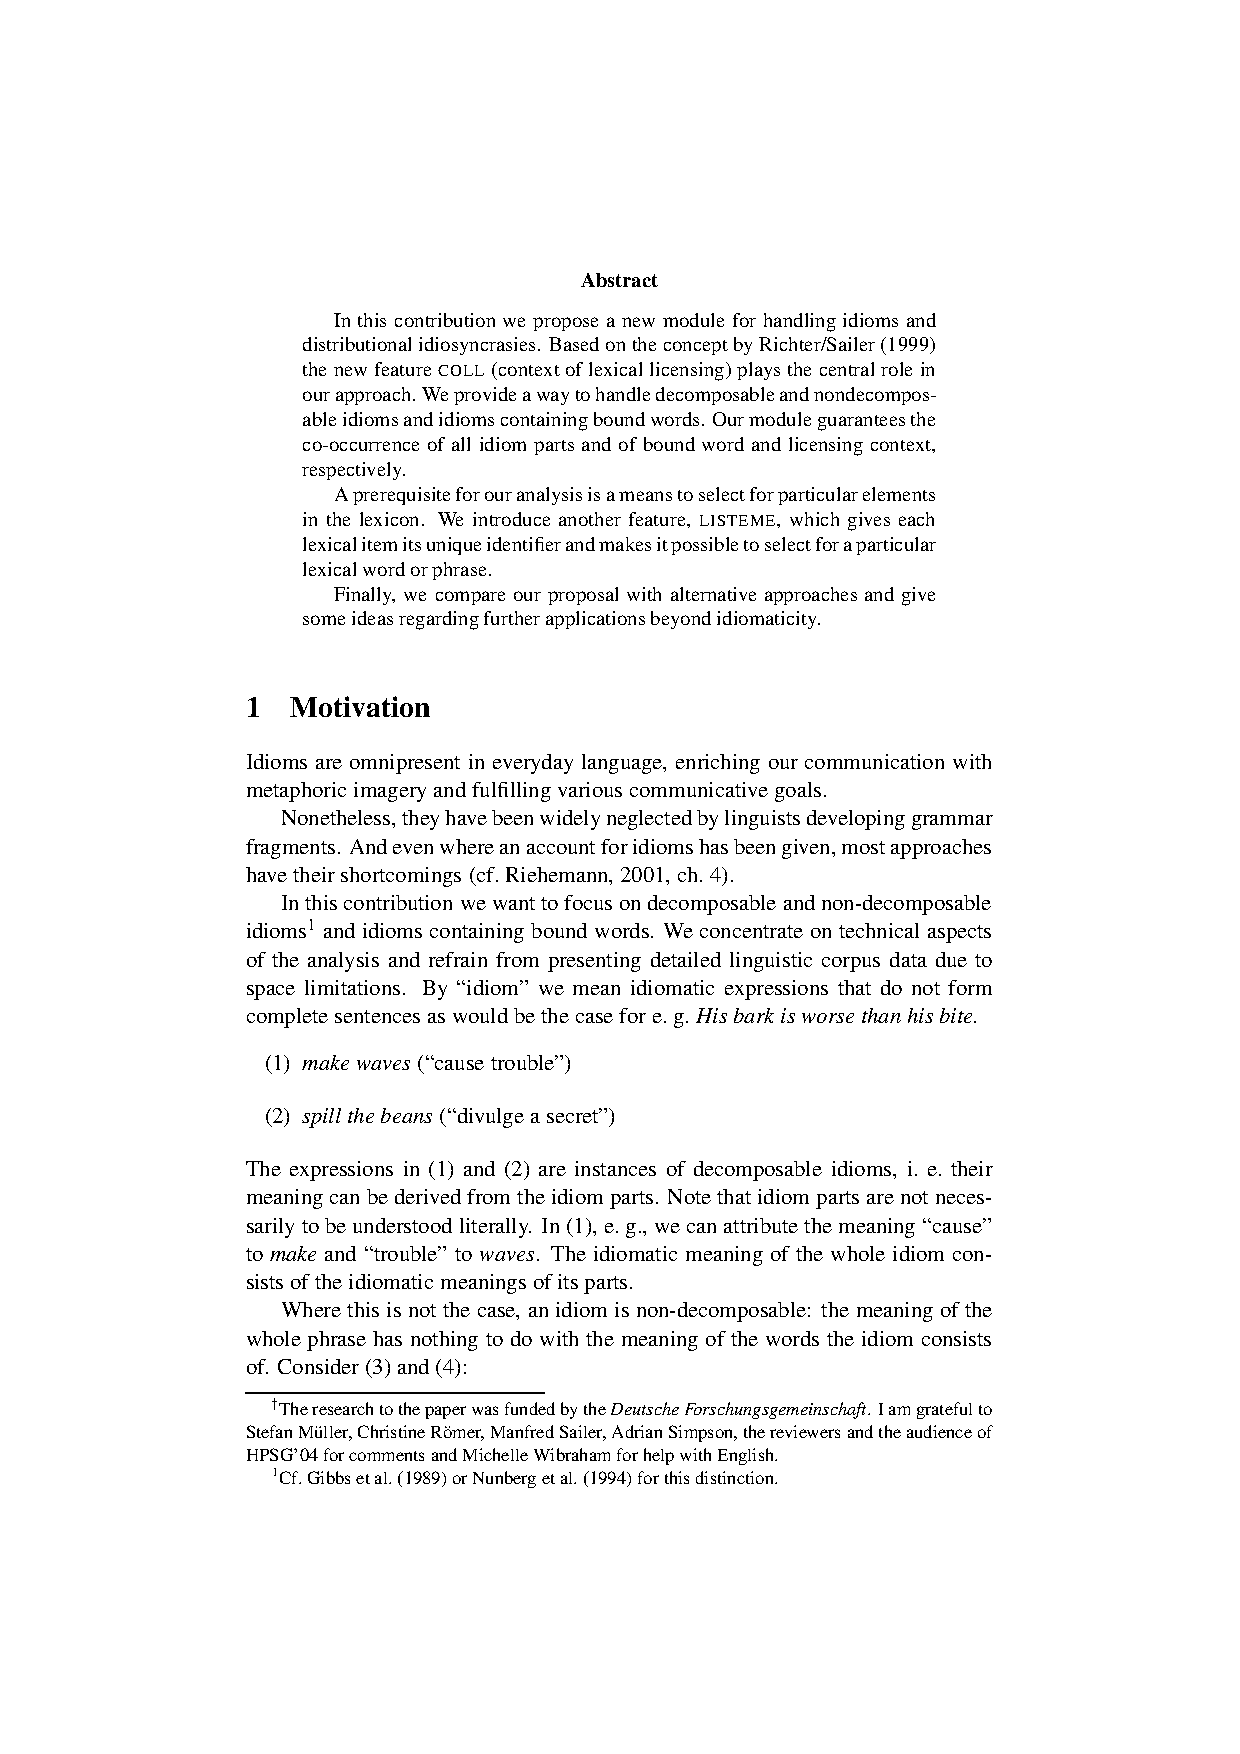
\includepdf[pages=-,pagecommand=\thispagestyle{plain}]{Includes/soehn.pdf}
        \setcounter{page}{274}
        \phantomsection
        \addcontentsline{toc}{section}{Mehran A. Taghvaipour: An HPSG Analysis of Persian Relative Clauses}
\thispagestyle{empty}

\begin{center}
  {\huge\bfseries An HPSG Analysis of Persian Relative Clauses\par}

  \bigskip

~\\
\begingroup
\setlength{\leftskip}{0pt plus 1fill}
\setlength{\rightskip}{0pt plus 1fill}
\setlength{\parindent}{0pt}
\setlength{\parfillskip}{0pt}
  \formatauthor{Mehran A. Taghvaipour}{\begin{tabular}{@{}c@{}}University of Essex\end{tabular}}

\par\endgroup

  \vspace*{8ex}

  Proceedings of the 11th International Conference on\par Head-Driven Phrase Structure Grammar

  \bigskip

  Center for Computational Linguistics, Katholieke Universiteit Leuven

  \medskip

  Stefan Müller (Editor)

  \medskip

  2004

  \medskip

  CSLI Publications

  \medskip

  pages 274--293

  \medskip

  \url{http://csli-publications.stanford.edu/HPSG/2004}
\end{center}
\vfill

\noindent



\vfill
\noindent
% APA Style
Taghvaipour, Mehran A. 2004. An HPSG Analysis of Persian Relative Clauses. In Müller, Stefan (Ed.), \emph{{Proceedings of the 11th International Conference on Head-Driven Phrase Structure Grammar, Center for Computational Linguistics, Katholieke Universiteit Leuven}}, 274--293. Stanford,
CA: CSLI Publications. \hfill\href{http://creativecommons.org/licenses/by/4.0/}{\includegraphics[height=.75em]{Includes/ccby.eps}}

\newpage
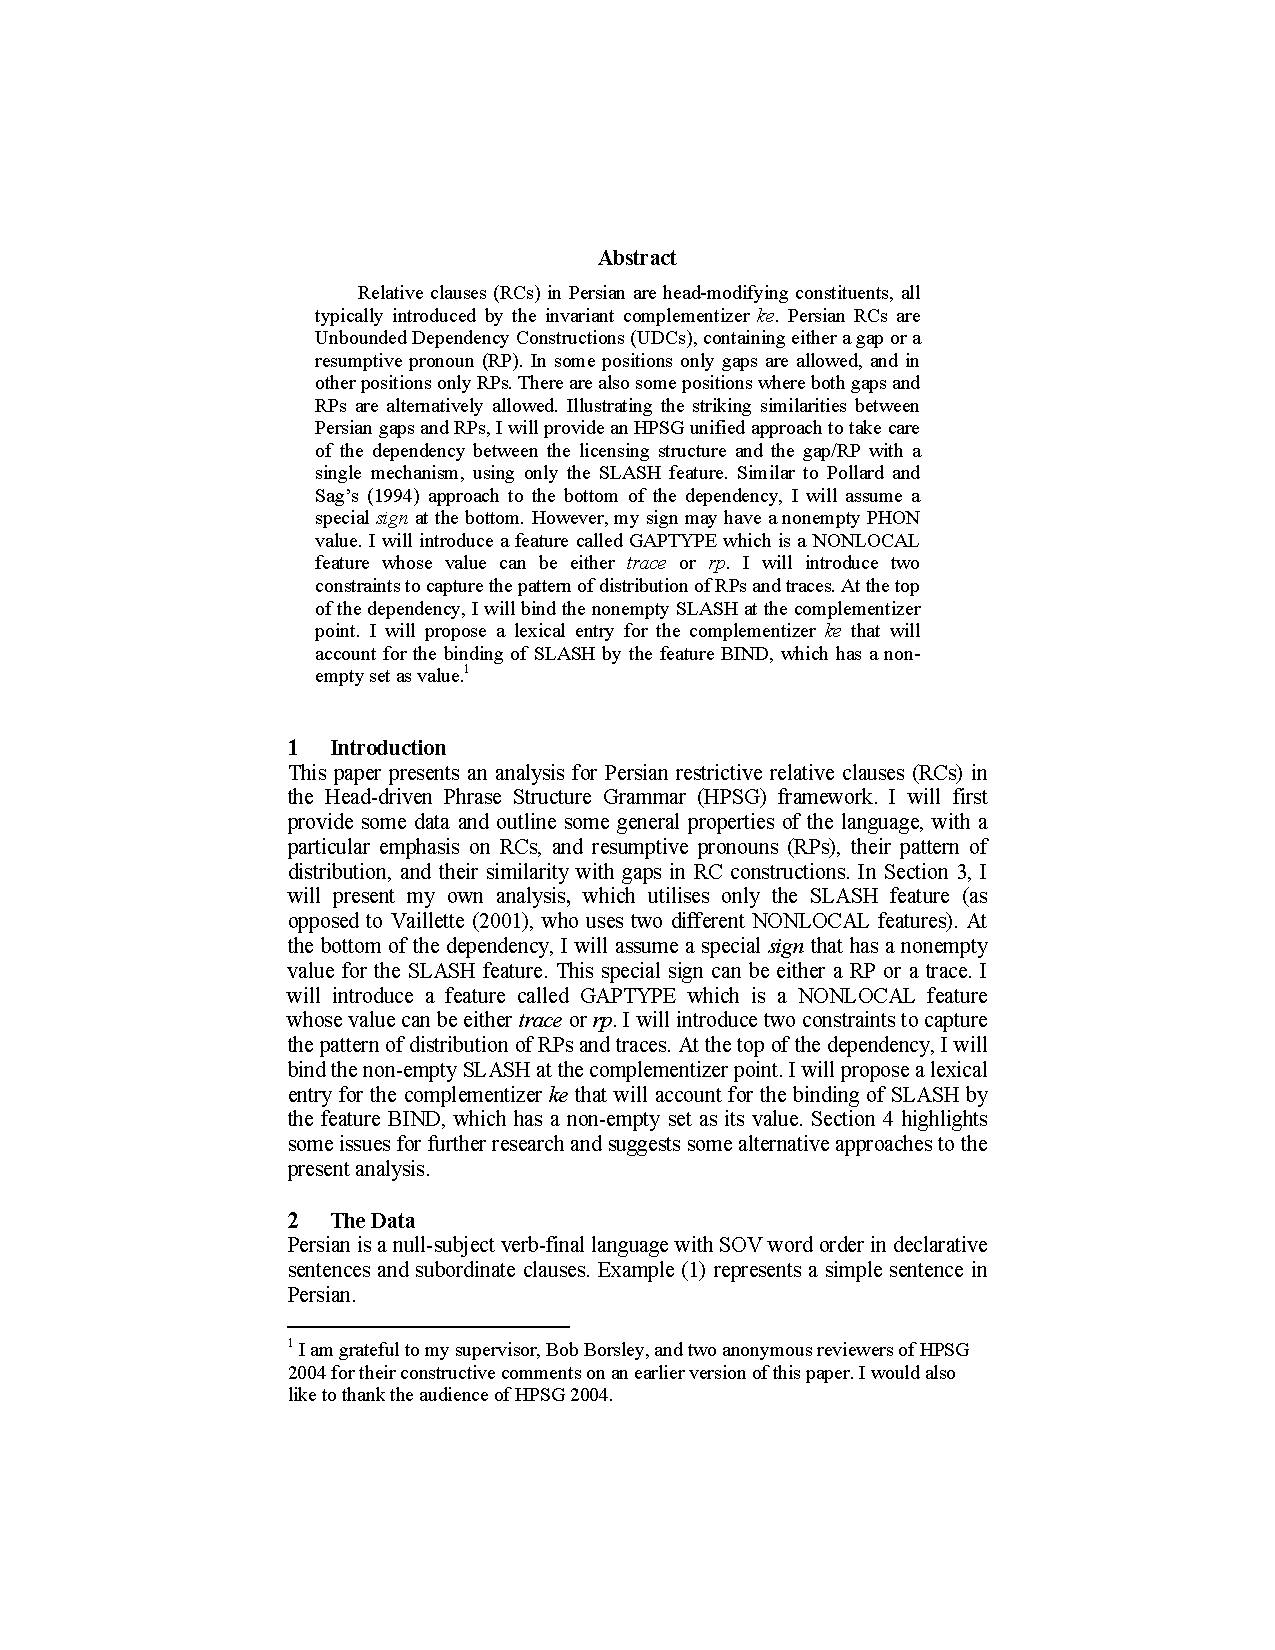
\includepdf[pages=-,pagecommand=\thispagestyle{plain}]{Includes/taghvaipour.pdf}
        \setcounter{page}{294}
        \phantomsection
        \addcontentsline{toc}{section}{Beata Trawinski: Towards Licensing of Adverbial Noun Phrases in HPSG}
\thispagestyle{empty}

\begin{center}
  {\huge\bfseries Towards Licensing of Adverbial Noun Phrases in HPSG\par}

  \bigskip

~\\
\begingroup
\setlength{\leftskip}{0pt plus 1fill}
\setlength{\rightskip}{0pt plus 1fill}
\setlength{\parindent}{0pt}
\setlength{\parfillskip}{0pt}
  \formatauthor{Beata Trawinski}{\begin{tabular}{@{}c@{}}University of Tübingen\end{tabular}}

\par\endgroup

  \vspace*{8ex}

  Proceedings of the 11th International Conference on\par Head-Driven Phrase Structure Grammar

  \bigskip

  Center for Computational Linguistics, Katholieke Universiteit Leuven

  \medskip

  Stefan Müller (Editor)

  \medskip

  2004

  \medskip

  CSLI Publications

  \medskip

  pages 294--312

  \medskip

  \url{http://csli-publications.stanford.edu/HPSG/2004}
\end{center}
\vfill

\noindent



\vfill
\noindent
% APA Style
Trawinski, Beata. 2004. Towards Licensing of Adverbial Noun Phrases in HPSG. In Müller, Stefan (Ed.), \emph{{Proceedings of the 11th International Conference on Head-Driven Phrase Structure Grammar, Center for Computational Linguistics, Katholieke Universiteit Leuven}}, 294--312. Stanford,
CA: CSLI Publications. \hfill\href{http://creativecommons.org/licenses/by/4.0/}{\includegraphics[height=.75em]{Includes/ccby.eps}}

\newpage
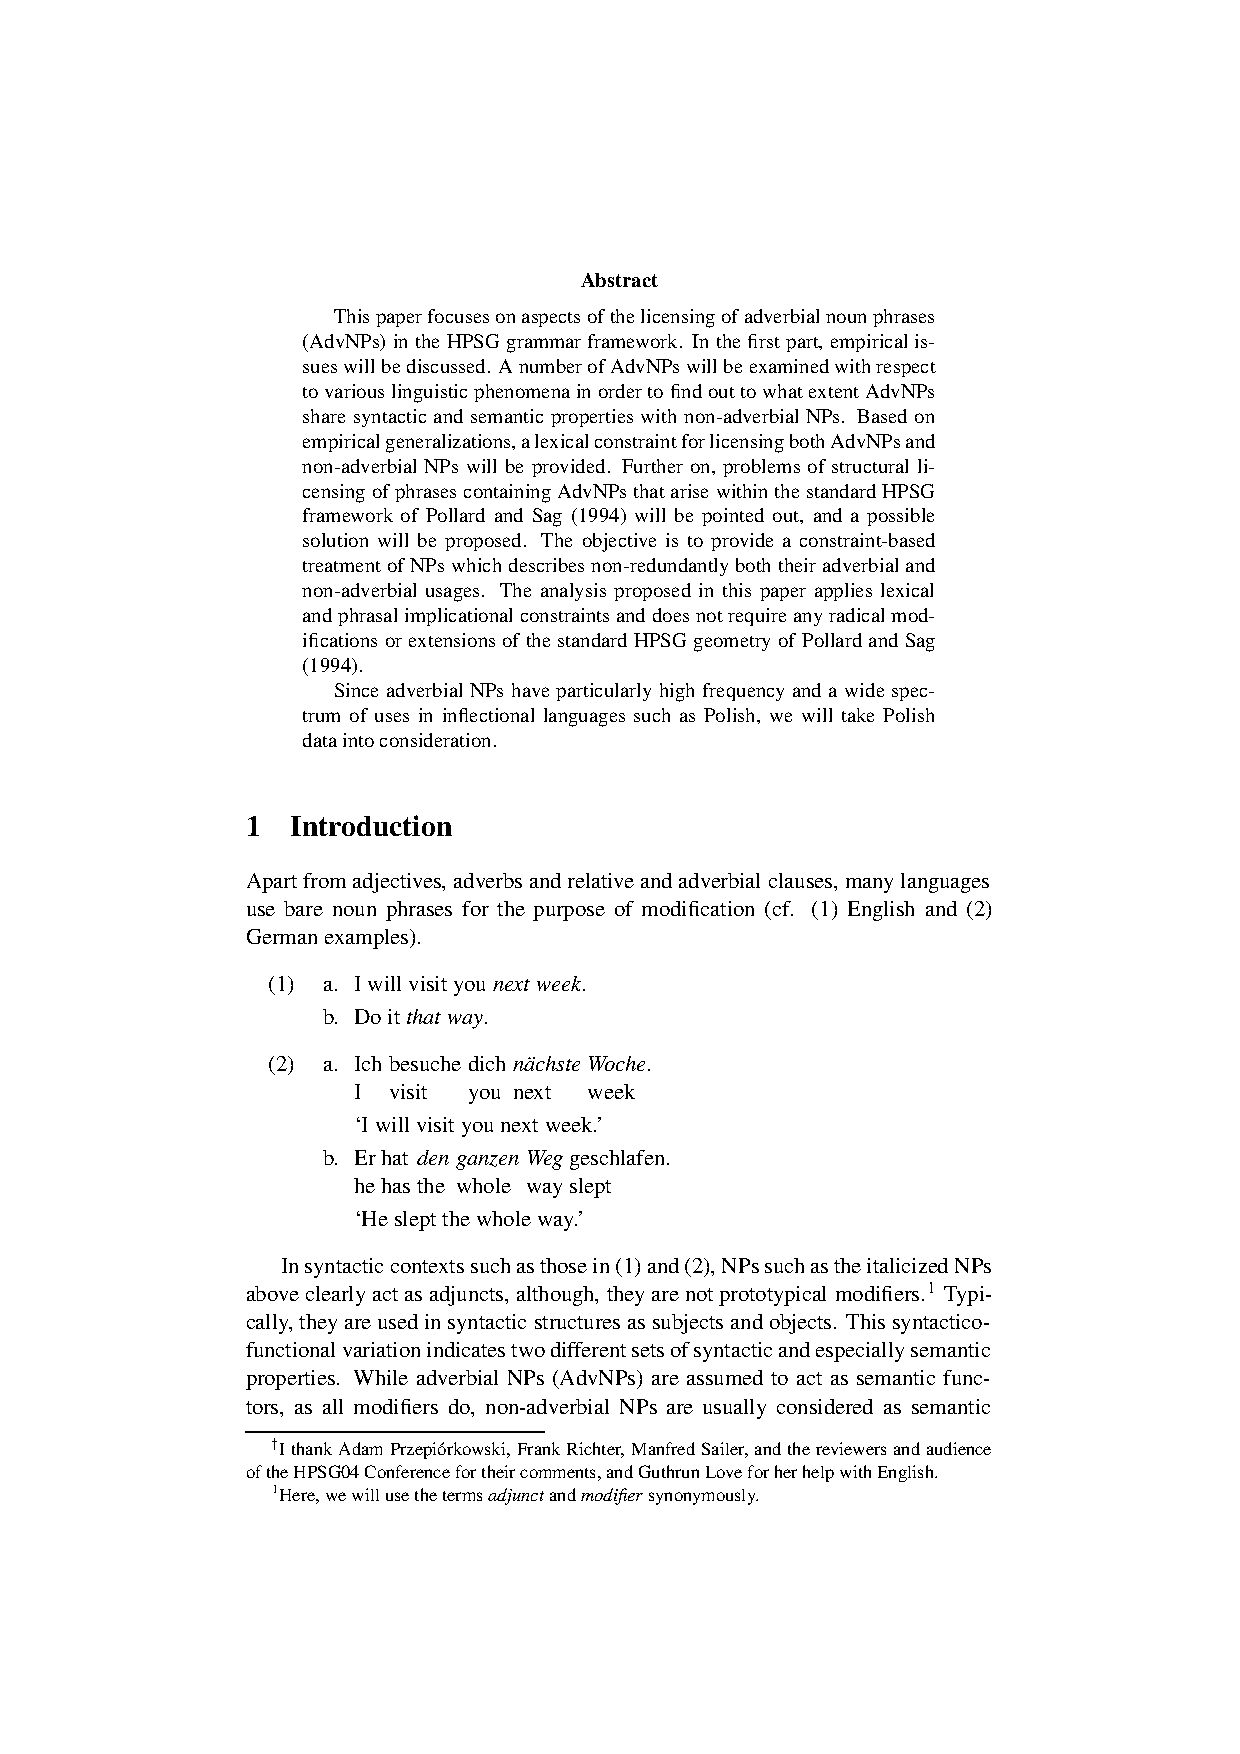
\includepdf[pages=-,pagecommand=\thispagestyle{plain}]{Includes/trawinski.pdf}
        \setcounter{page}{313}
        \phantomsection
        \addcontentsline{toc}{section}{Frank Van Eynde: Pied Piping is a Local Dependency}
\thispagestyle{empty}

\begin{center}
  {\huge\bfseries Pied Piping is a Local Dependency\par}

  \bigskip

~\\
\begingroup
\setlength{\leftskip}{0pt plus 1fill}
\setlength{\rightskip}{0pt plus 1fill}
\setlength{\parindent}{0pt}
\setlength{\parfillskip}{0pt}
  \formatauthor{Frank Van Eynde}{\begin{tabular}{@{}c@{}}Universiteit Leuven\end{tabular}}

\par\endgroup

  \vspace*{8ex}

  Proceedings of the 11th International Conference on\par Head-Driven Phrase Structure Grammar

  \bigskip

  Center for Computational Linguistics, Katholieke Universiteit Leuven

  \medskip

  Stefan Müller (Editor)

  \medskip

  2004

  \medskip

  CSLI Publications

  \medskip

  pages 313--334

  \medskip

  \url{http://csli-publications.stanford.edu/HPSG/2004}
\end{center}
\vfill

\noindent



\vfill
\noindent
% APA Style
Van Eynde, Frank. 2004. Pied Piping is a Local Dependency. In Müller, Stefan (Ed.), \emph{{Proceedings of the 11th International Conference on Head-Driven Phrase Structure Grammar, Center for Computational Linguistics, Katholieke Universiteit Leuven}}, 313--334. Stanford,
CA: CSLI Publications. \hfill\href{http://creativecommons.org/licenses/by/4.0/}{\includegraphics[height=.75em]{Includes/ccby.eps}}

\newpage
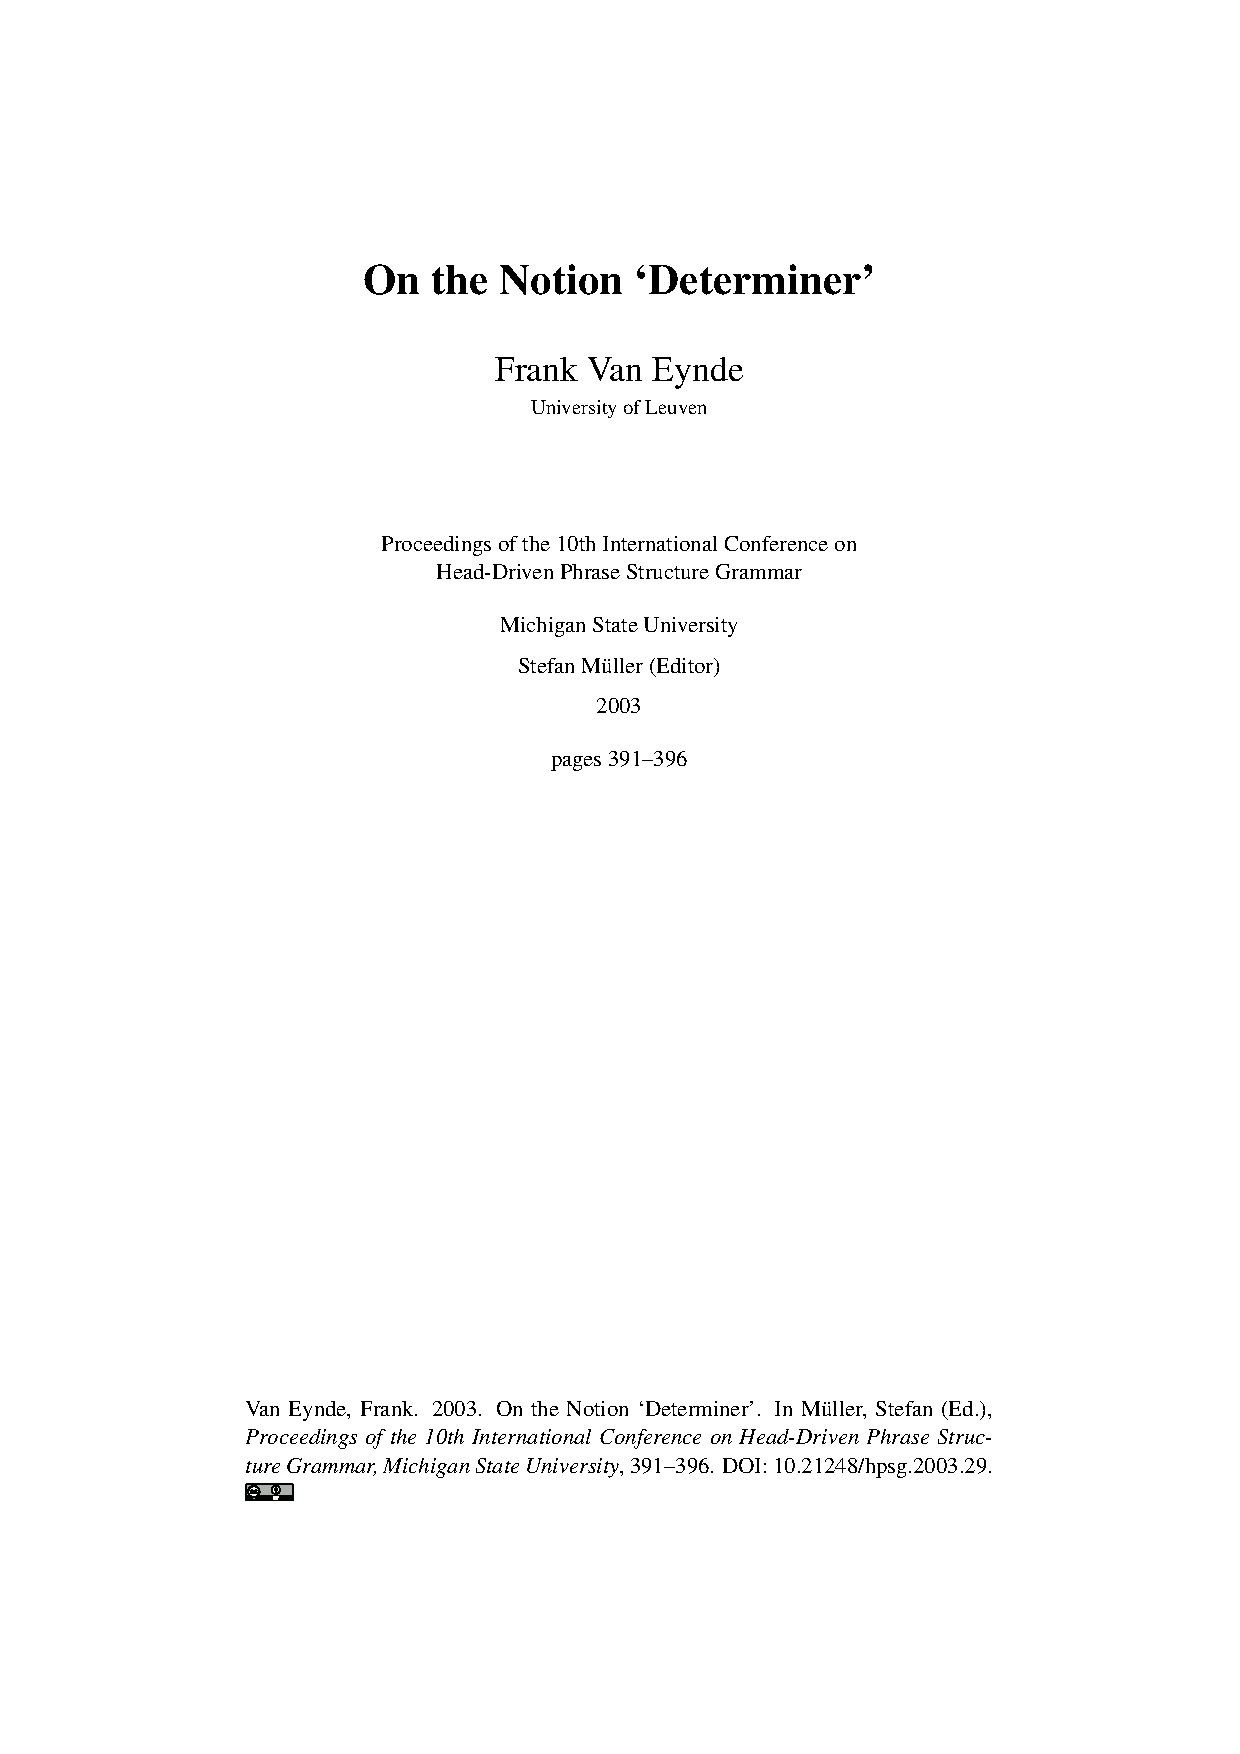
\includepdf[pages=-,pagecommand=\thispagestyle{plain}]{Includes/vaneynde.pdf}
        \setcounter{page}{335}
        \phantomsection
        \addcontentsline{toc}{section}{Sh{\^u}ichi Yatabe: A Comprehensive Theory of Coordination of Unlikes}
\thispagestyle{empty}

\begin{center}
  {\huge\bfseries A Comprehensive Theory of Coordination of Unlikes\par}

  \bigskip

~\\
\begingroup
\setlength{\leftskip}{0pt plus 1fill}
\setlength{\rightskip}{0pt plus 1fill}
\setlength{\parindent}{0pt}
\setlength{\parfillskip}{0pt}
  \formatauthor{Shûichi Yatabe}{\begin{tabular}{@{}c@{}}University of Tokyo\end{tabular}}

\par\endgroup

  \vspace*{8ex}

  Proceedings of the 11th International Conference on\par Head-Driven Phrase Structure Grammar

  \bigskip

  Center for Computational Linguistics, Katholieke Universiteit Leuven

  \medskip

  Stefan Müller (Editor)

  \medskip

  2004

  \medskip

  CSLI Publications

  \medskip

  pages 335--355

  \medskip

  \url{http://csli-publications.stanford.edu/HPSG/2004}
\end{center}
\vfill

\noindent



\vfill
\noindent
% APA Style
Yatabe, Shûichi. 2004. A Comprehensive Theory of Coordination of Unlikes. In Müller, Stefan (Ed.), \emph{{Proceedings of the 11th International Conference on Head-Driven Phrase Structure Grammar, Center for Computational Linguistics, Katholieke Universiteit Leuven}}, 335--355. Stanford,
CA: CSLI Publications. \hfill\href{http://creativecommons.org/licenses/by/4.0/}{\includegraphics[height=.75em]{Includes/ccby.eps}}

\newpage
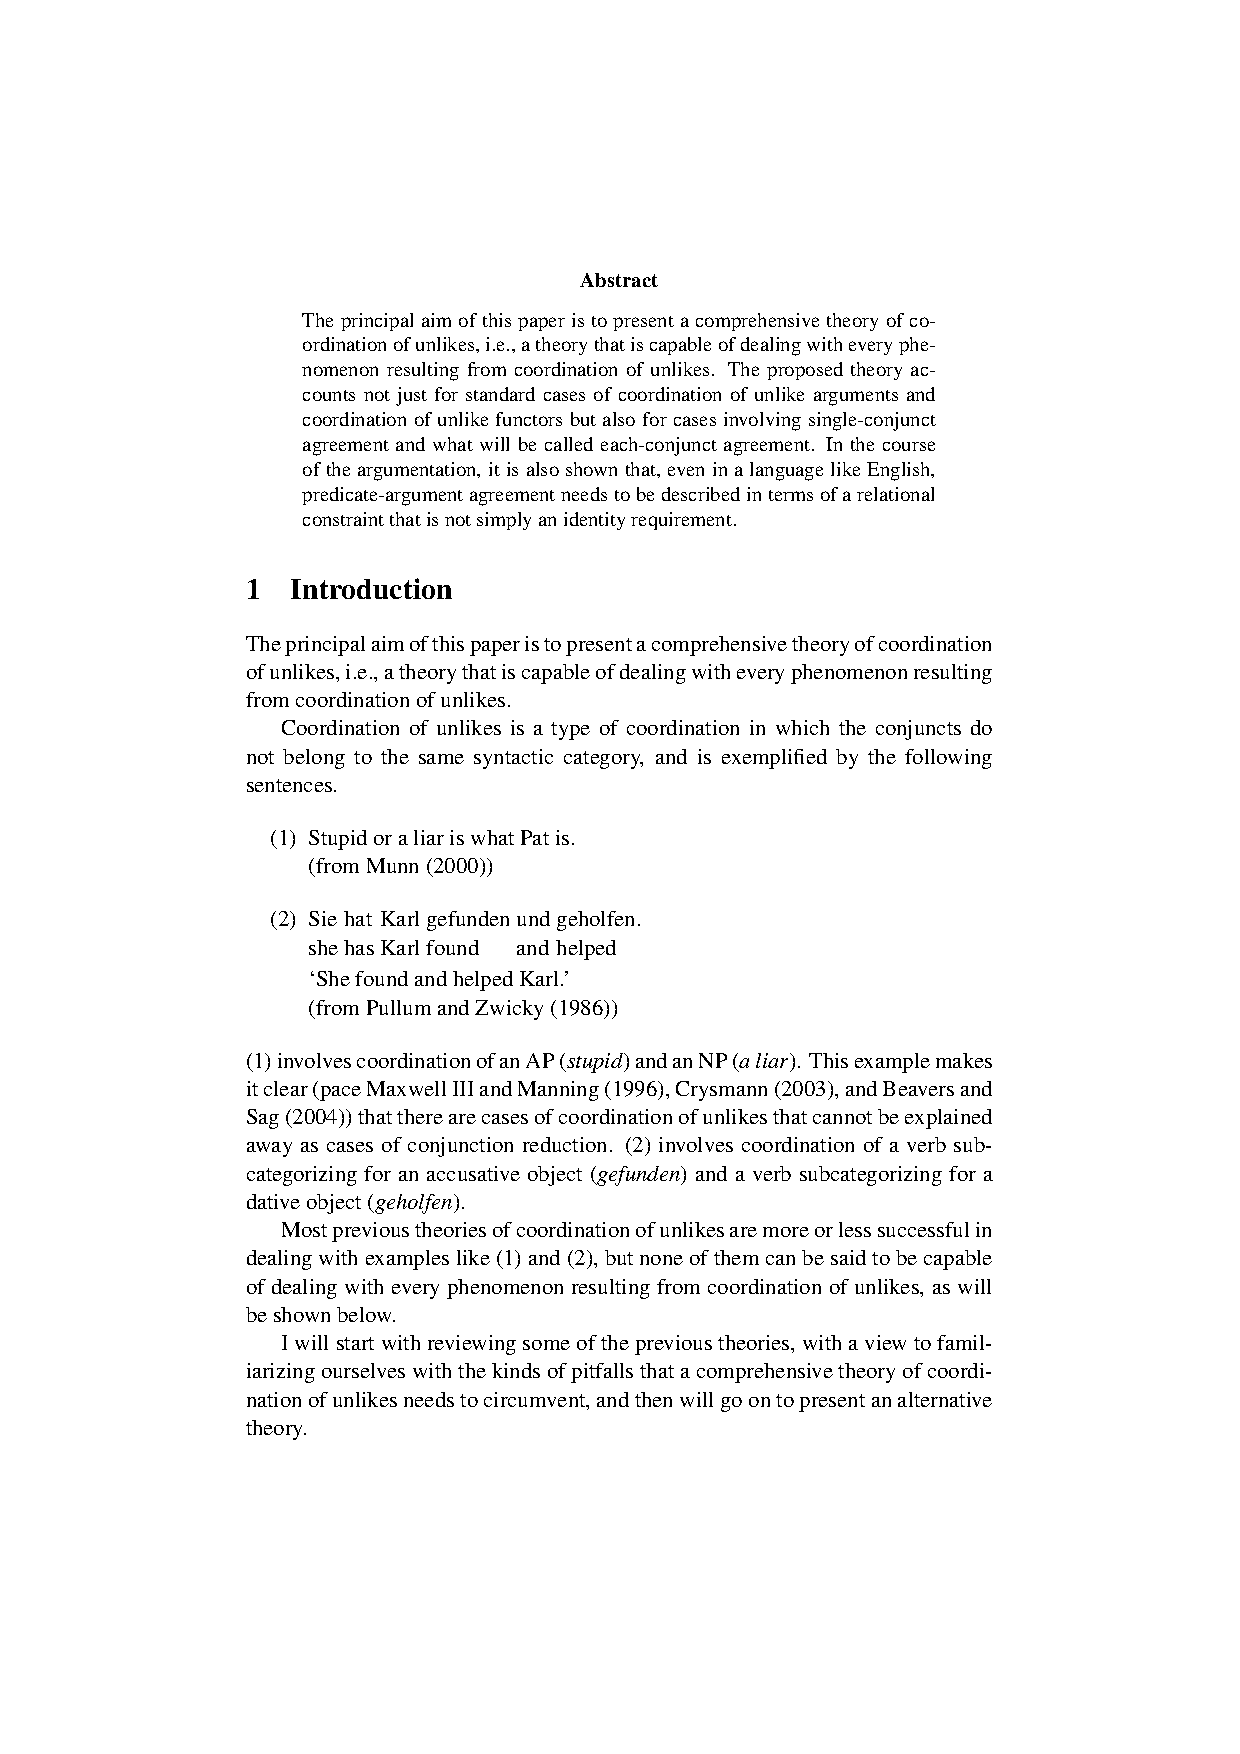
\includepdf[pages=-,pagecommand=\thispagestyle{plain}]{Includes/yatabe.pdf}
\part{Contributions to the Workshop}
\thispagestyle{empty}
\newpage
        \setcounter{page}{357}
        \phantomsection
        \addcontentsline{toc}{section}{Dorothee Beermann, Lars Hellan: A treatment of directionals in implemented HPSG Grammars}
\thispagestyle{empty}

\begin{center}
  {\huge\bfseries A treatment of directionals in implemented HPSG Grammars\par}

  \bigskip

~\\
\begingroup
\setlength{\leftskip}{0pt plus 1fill}
\setlength{\rightskip}{0pt plus 1fill}
\setlength{\parindent}{0pt}
\setlength{\parfillskip}{0pt}
  \formatauthor{Dorothee Beermann}{\begin{tabular}{@{}c@{}}NTNU Trondheim\end{tabular}}
\formatauthor{Lars Hellan}{\begin{tabular}{@{}c@{}}NTNU Trondheim\end{tabular}}

\par\endgroup

  \vspace*{8ex}

  Proceedings of the 11th International Conference on\par Head-Driven Phrase Structure Grammar

  \bigskip

  Center for Computational Linguistics, Katholieke Universiteit Leuven

  \medskip

  Stefan Müller (Editor)

  \medskip

  2004

  \medskip

  CSLI Publications

  \medskip

  pages 357--377

  \medskip

  \url{http://csli-publications.stanford.edu/HPSG/2004}
\end{center}
\vfill

\noindent



\vfill
\noindent
% APA Style
Beermann, Dorothee, \& Hellan, Lars. 2004. A treatment of directionals in implemented HPSG Grammars. In Müller, Stefan (Ed.), \emph{{Proceedings of the 11th International Conference on Head-Driven Phrase Structure Grammar, Center for Computational Linguistics, Katholieke Universiteit Leuven}}, 357--377. Stanford,
CA: CSLI Publications. \hfill\href{http://creativecommons.org/licenses/by/4.0/}{\includegraphics[height=.75em]{Includes/ccby.eps}}

\newpage
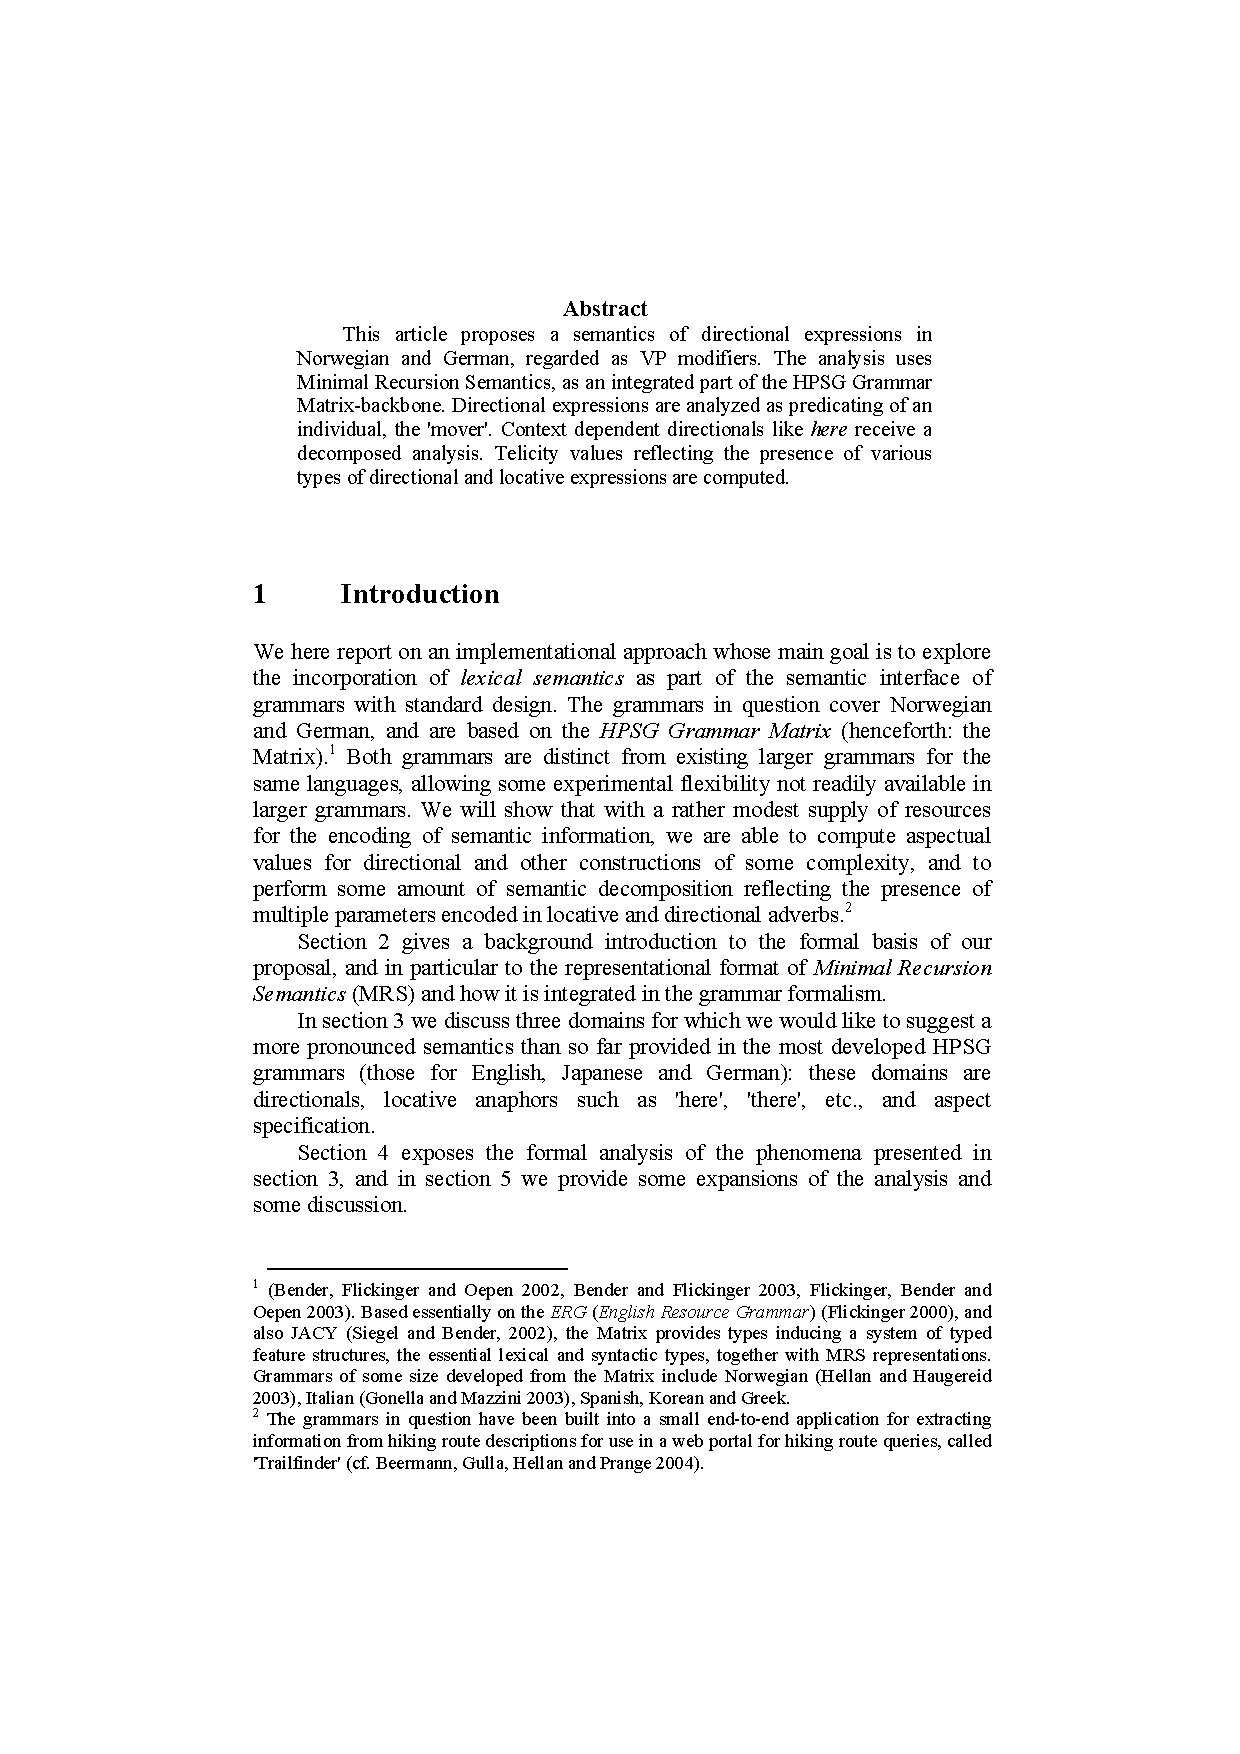
\includepdf[pages=-,pagecommand=\thispagestyle{plain}]{Includes/beermann-hellan.pdf}
        \setcounter{page}{378}
        \phantomsection
        \addcontentsline{toc}{section}{Berthold Crysmann: Underspecification of Intersective Modifier Attachment: Some Arguments from German}
\thispagestyle{empty}

\begin{center}
  {\huge\bfseries Underspecification of Intersective Modifier Attachment: Some Arguments from German\par}

  \bigskip

~\\
\begingroup
\setlength{\leftskip}{0pt plus 1fill}
\setlength{\rightskip}{0pt plus 1fill}
\setlength{\parindent}{0pt}
\setlength{\parfillskip}{0pt}
  \formatauthor{Berthold Crysmann}{\begin{tabular}{@{}c@{}}DFKI, Saarland University\end{tabular}}

\par\endgroup

  \vspace*{8ex}

  Proceedings of the 11th International Conference on\par Head-Driven Phrase Structure Grammar

  \bigskip

  Center for Computational Linguistics, Katholieke Universiteit Leuven

  \medskip

  Stefan Müller (Editor)

  \medskip

  2004

  \medskip

  CSLI Publications

  \medskip

  pages 378--392

  \medskip

  \url{http://csli-publications.stanford.edu/HPSG/2004}
\end{center}
\vfill

\noindent



\vfill
\noindent
% APA Style
Crysmann, Berthold. 2004. Underspecification of Intersective Modifier Attachment: Some Arguments from German. In Müller, Stefan (Ed.), \emph{{Proceedings of the 11th International Conference on Head-Driven Phrase Structure Grammar, Center for Computational Linguistics, Katholieke Universiteit Leuven}}, 378--392. Stanford,
CA: CSLI Publications. \hfill\href{http://creativecommons.org/licenses/by/4.0/}{\includegraphics[height=.75em]{Includes/ccby.eps}}

\newpage
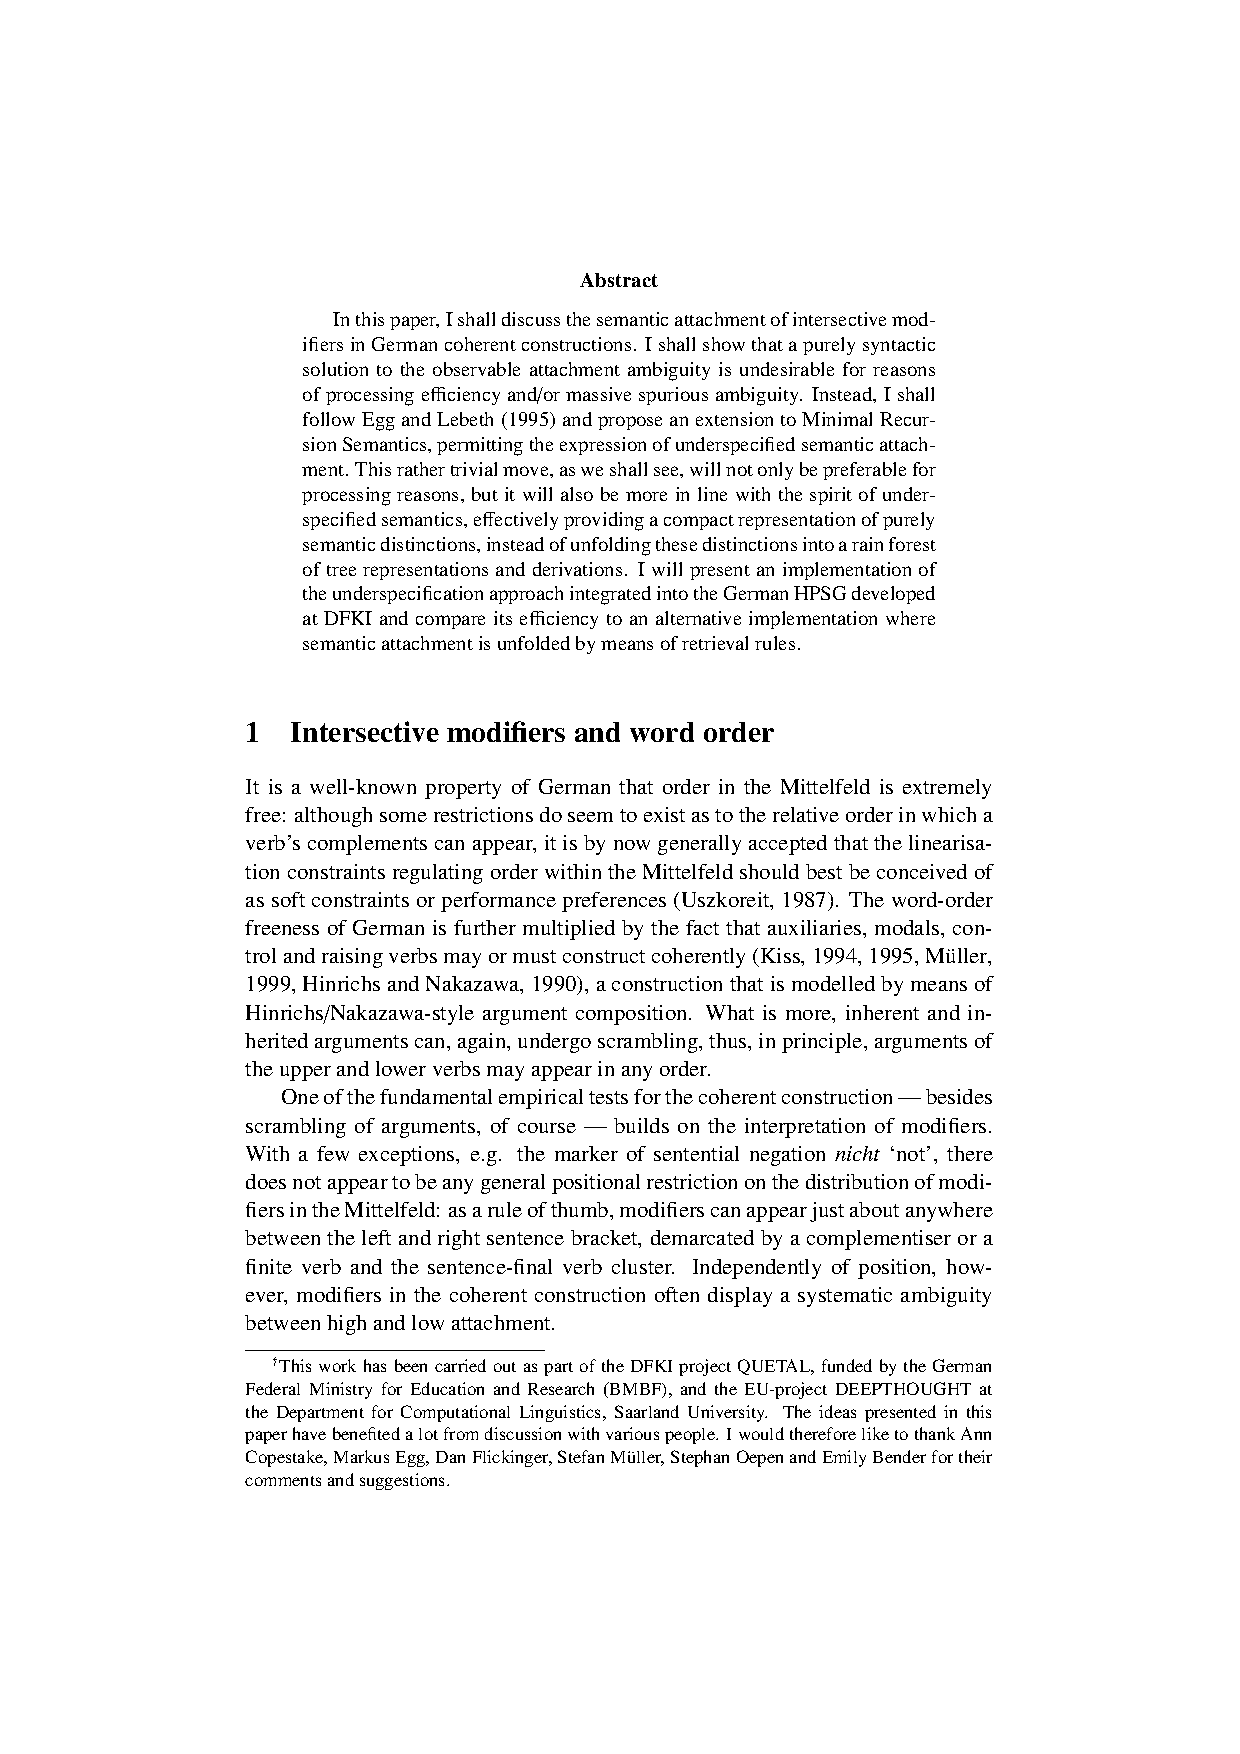
\includepdf[pages=-,pagecommand=\thispagestyle{plain}]{Includes/crysmann.pdf}
        \setcounter{page}{393}
        \phantomsection
        \addcontentsline{toc}{section}{Anette Frank, Kathrin Spreyer, Witold Dro\.zd\.zy\'nski, Hans-Ulrich Krieger, Ulrich Sch\"{a}fer: Constraint-Based RMRS Construction from Shallow Grammars}
\thispagestyle{empty}

\begin{center}
  {\huge\bfseries Constraint-Based RMRS Construction from Shallow Grammars\par}

  \bigskip

~\\
\begingroup
\setlength{\leftskip}{0pt plus 1fill}
\setlength{\rightskip}{0pt plus 1fill}
\setlength{\parindent}{0pt}
\setlength{\parfillskip}{0pt}
  \formatauthor{Anette Frank}{\begin{tabular}{@{}c@{}}DFKI Saarbrücken\end{tabular}}
\formatauthor{Kathrin Spreyer}{\begin{tabular}{@{}c@{}}DFKI Saarbrücken\end{tabular}}
\formatauthor{Witold Drożdżyński}{\begin{tabular}{@{}c@{}}DFKI Saarbrücken\end{tabular}}
\formatauthor{Hans-Ulrich Krieger}{\begin{tabular}{@{}c@{}}DFKI Saarbrücken\end{tabular}}
\formatauthor{Ulrich Schäfer}{\begin{tabular}{@{}c@{}}DFKI Saarbrücken\end{tabular}}

\par\endgroup

  \vspace*{8ex}

  Proceedings of the 11th International Conference on\par Head-Driven Phrase Structure Grammar

  \bigskip

  Center for Computational Linguistics, Katholieke Universiteit Leuven

  \medskip

  Stefan Müller (Editor)

  \medskip

  2004

  \medskip

  CSLI Publications

  \medskip

  pages 393--413

  \medskip

  \url{http://csli-publications.stanford.edu/HPSG/2004}
\end{center}
\vfill

\noindent



\vfill
\noindent
% APA Style
Frank, Anette, Spreyer, Kathrin, Drożdżyński, Witold, Krieger, Hans-Ulrich, \& Schäfer, Ulrich. 2004. Constraint-Based RMRS Construction from Shallow Grammars. In Müller, Stefan (Ed.), \emph{{Proceedings of the 11th International Conference on Head-Driven Phrase Structure Grammar, Center for Computational Linguistics, Katholieke Universiteit Leuven}}, 393--413. Stanford,
CA: CSLI Publications. \hfill\href{http://creativecommons.org/licenses/by/4.0/}{\includegraphics[height=.75em]{Includes/ccby.eps}}

\newpage
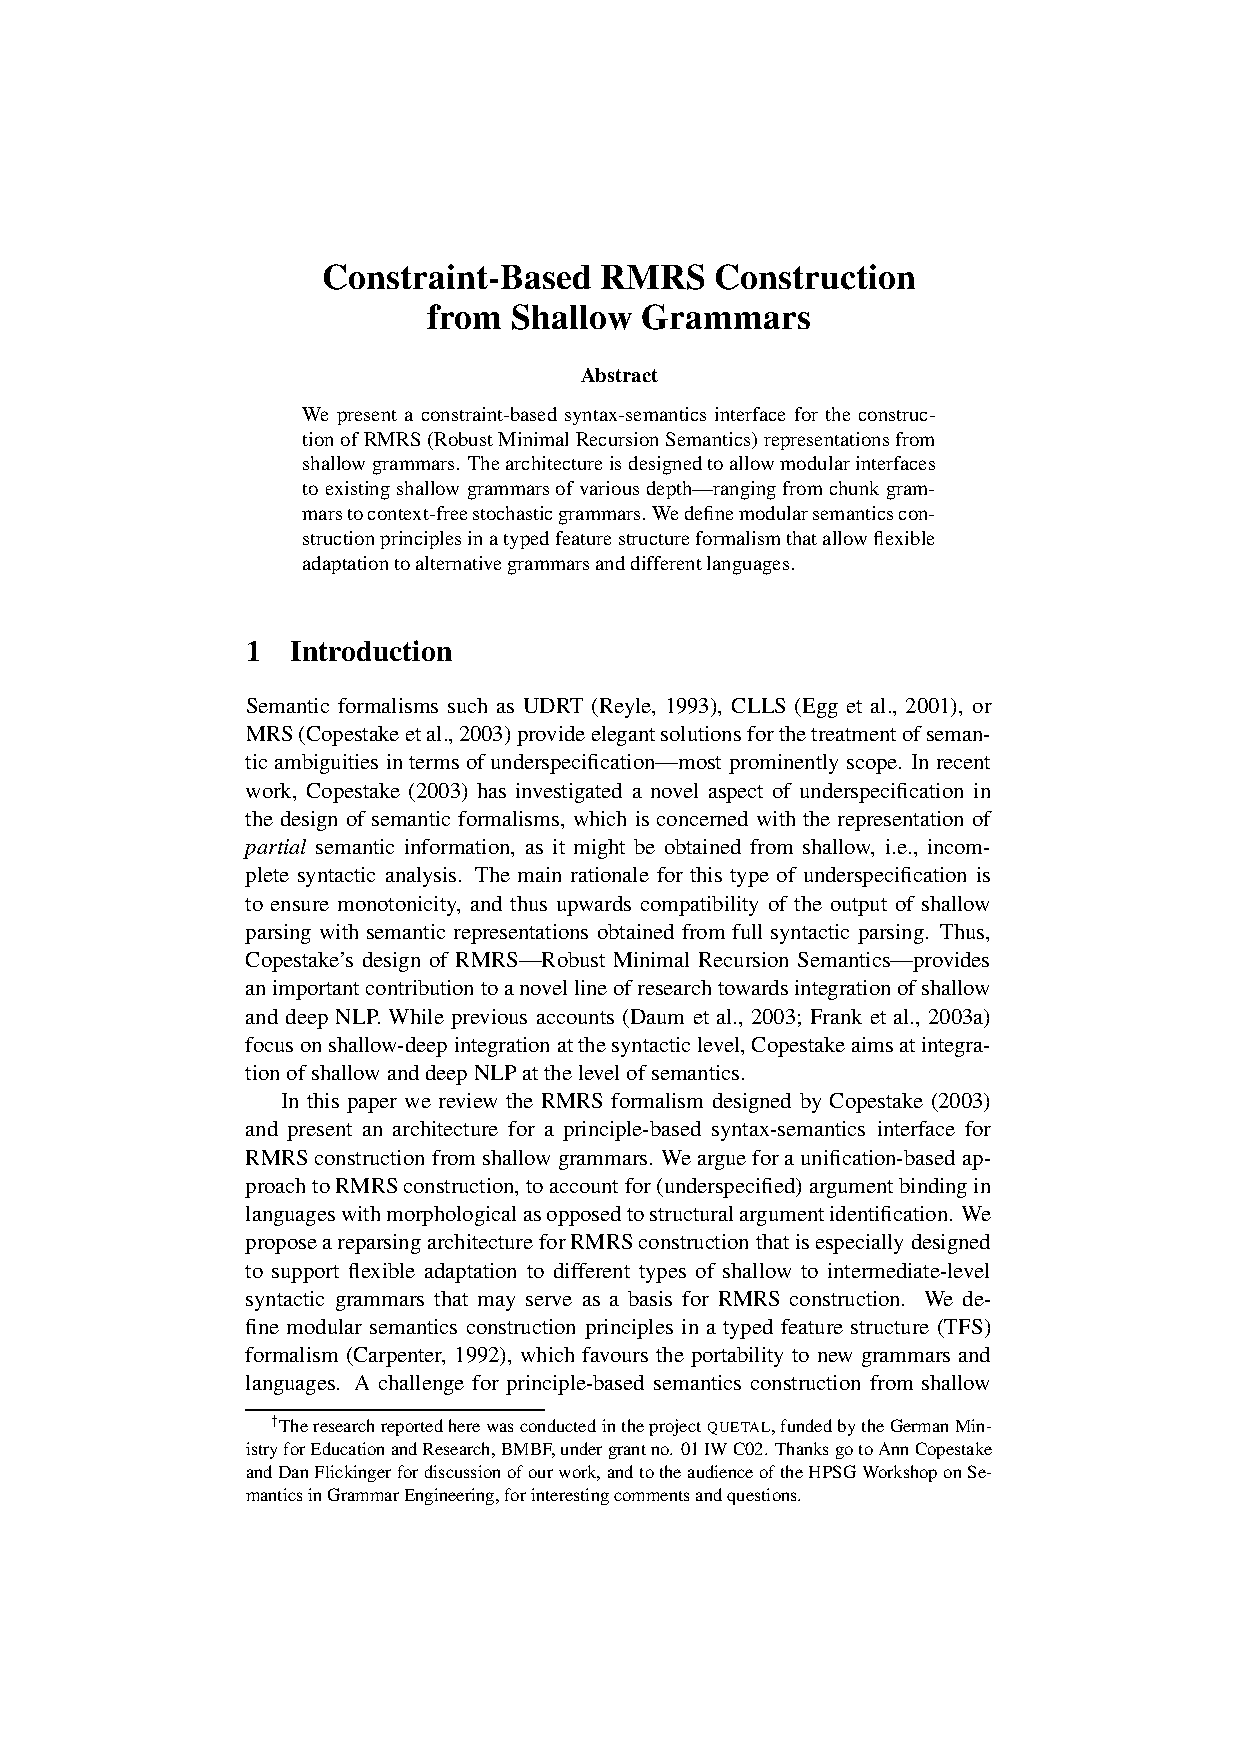
\includepdf[pages=-,pagecommand=\thispagestyle{plain}]{Includes/fsdks.pdf}
        \setcounter{page}{414}
        \phantomsection
        \addcontentsline{toc}{section}{Petter Haugereid: Linking in Constructions}
\thispagestyle{empty}

\begin{center}
  {\huge\bfseries Linking in Constructions\par}

  \bigskip

~\\
\begingroup
\setlength{\leftskip}{0pt plus 1fill}
\setlength{\rightskip}{0pt plus 1fill}
\setlength{\parindent}{0pt}
\setlength{\parfillskip}{0pt}
  \formatauthor{Petter Haugereid}{\begin{tabular}{@{}c@{}}NTNU Trondheim\end{tabular}}

\par\endgroup

  \vspace*{8ex}

  Proceedings of the 11th International Conference on\par Head-Driven Phrase Structure Grammar

  \bigskip

  Center for Computational Linguistics, Katholieke Universiteit Leuven

  \medskip

  Stefan Müller (Editor)

  \medskip

  2004

  \medskip

  CSLI Publications

  \medskip

  pages 414--422

  \medskip

  \url{http://csli-publications.stanford.edu/HPSG/2004}
\end{center}
\vfill

\noindent



\vfill
\noindent
% APA Style
Haugereid, Petter. 2004. Linking in Constructions. In Müller, Stefan (Ed.), \emph{{Proceedings of the 11th International Conference on Head-Driven Phrase Structure Grammar, Center for Computational Linguistics, Katholieke Universiteit Leuven}}, 414--422. Stanford,
CA: CSLI Publications. \hfill\href{http://creativecommons.org/licenses/by/4.0/}{\includegraphics[height=.75em]{Includes/ccby.eps}}

\newpage
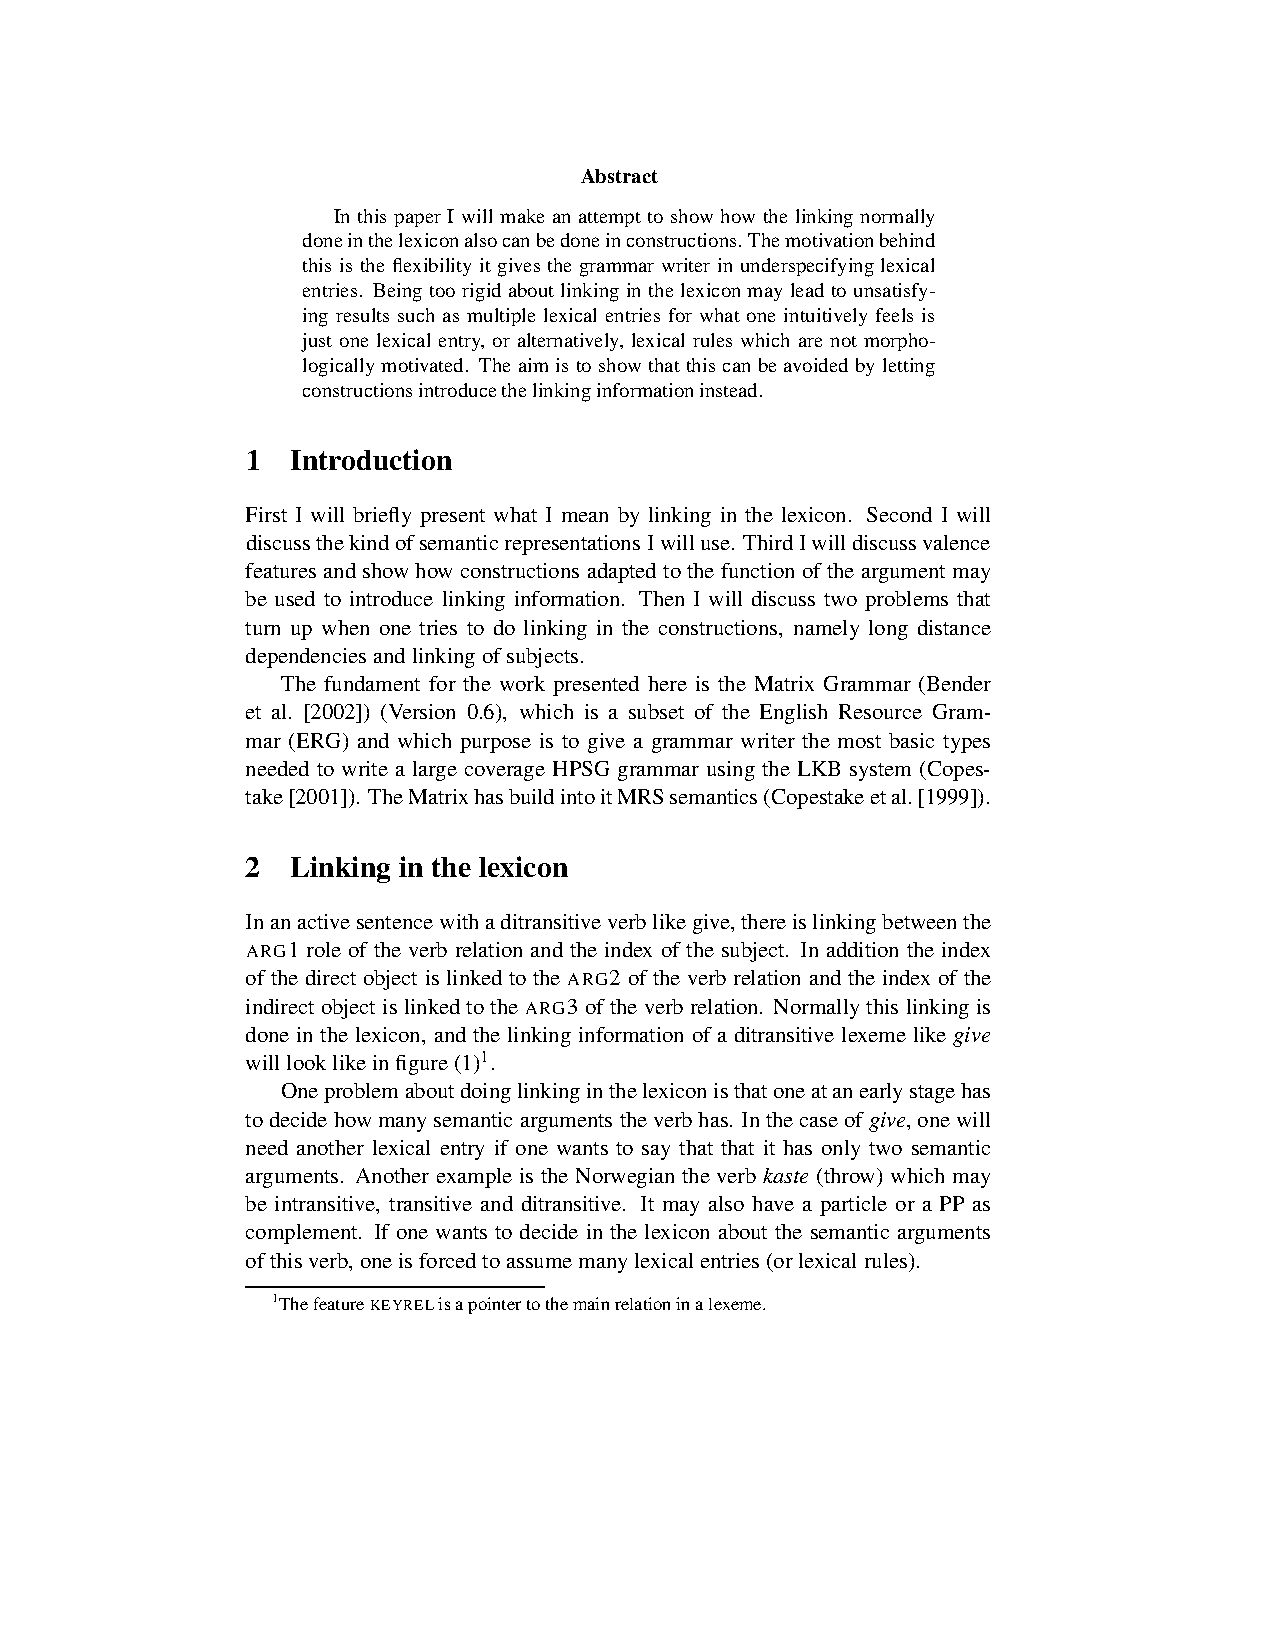
\includepdf[pages=-,pagecommand=\thispagestyle{plain}]{Includes/haugereid.pdf}
        \setcounter{page}{423}
        \phantomsection
        \addcontentsline{toc}{section}{Gerald Penn, Frank Richter: Lexical Resource Semantics: From Theory to Implementation}
\thispagestyle{empty}

\begin{center}
  {\huge\bfseries Lexical Resource Semantics: From Theory to Implementation\par}

  \bigskip

~\\
\begingroup
\setlength{\leftskip}{0pt plus 1fill}
\setlength{\rightskip}{0pt plus 1fill}
\setlength{\parindent}{0pt}
\setlength{\parfillskip}{0pt}
  \formatauthor{Gerald Penn}{\begin{tabular}{@{}c@{}}University of Toronto\end{tabular}}
\formatauthor{Frank Richter}{\begin{tabular}{@{}c@{}}Universität Tübingen\end{tabular}}

\par\endgroup

  \vspace*{8ex}

  Proceedings of the 11th International Conference on\par Head-Driven Phrase Structure Grammar

  \bigskip

  Center for Computational Linguistics, Katholieke Universiteit Leuven

  \medskip

  Stefan Müller (Editor)

  \medskip

  2004

  \medskip

  CSLI Publications

  \medskip

  pages 423--443

  \medskip

  \url{http://csli-publications.stanford.edu/HPSG/2004}
\end{center}
\vfill

\noindent



\vfill
\noindent
% APA Style
Penn, Gerald, \& Richter, Frank. 2004. Lexical Resource Semantics: From Theory to Implementation. In Müller, Stefan (Ed.), \emph{{Proceedings of the 11th International Conference on Head-Driven Phrase Structure Grammar, Center for Computational Linguistics, Katholieke Universiteit Leuven}}, 423--443. Stanford,
CA: CSLI Publications. \hfill\href{http://creativecommons.org/licenses/by/4.0/}{\includegraphics[height=.75em]{Includes/ccby.eps}}

\newpage
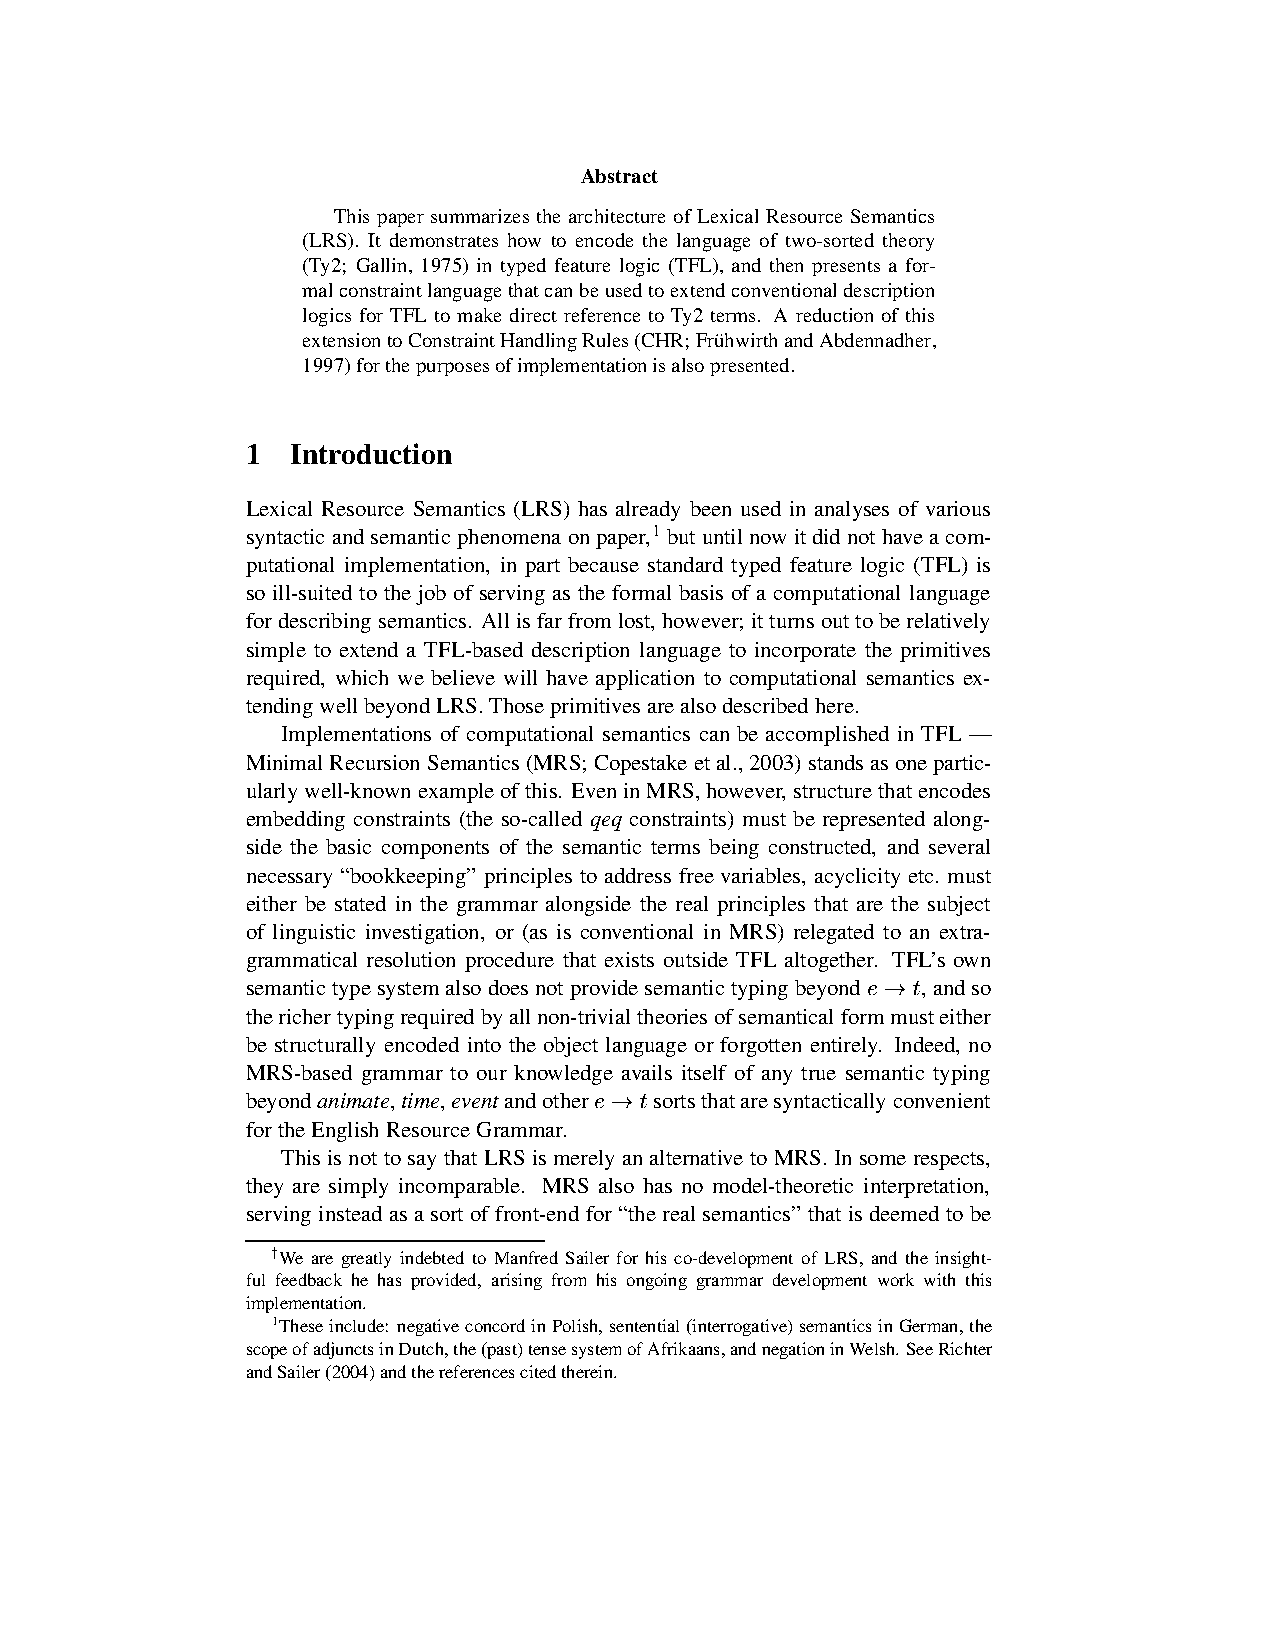
\includepdf[pages=-,pagecommand=\thispagestyle{plain}]{Includes/penn-richter.pdf}
        \setcounter{page}{444}
        \phantomsection
        \addcontentsline{toc}{section}{Anders S{\o}gaard: A Compound Matrix}
\thispagestyle{empty}

\begin{center}
  {\huge\bfseries A Compound Matrix\par}

  \bigskip

~\\
\begingroup
\setlength{\leftskip}{0pt plus 1fill}
\setlength{\rightskip}{0pt plus 1fill}
\setlength{\parindent}{0pt}
\setlength{\parfillskip}{0pt}
  \formatauthor{Anders Søgaard}{\begin{tabular}{@{}c@{}}Katholieke Universiteit Leuven\end{tabular}}

\par\endgroup

  \vspace*{8ex}

  Proceedings of the 11th International Conference on\par Head-Driven Phrase Structure Grammar

  \bigskip

  Center for Computational Linguistics, Katholieke Universiteit Leuven

  \medskip

  Stefan Müller (Editor)

  \medskip

  2004

  \medskip

  CSLI Publications

  \medskip

  pages 444--456

  \medskip

  \url{http://csli-publications.stanford.edu/HPSG/2004}
\end{center}
\vfill

\noindent



\vfill
\noindent
% APA Style
Søgaard, Anders. 2004. A Compound Matrix. In Müller, Stefan (Ed.), \emph{{Proceedings of the 11th International Conference on Head-Driven Phrase Structure Grammar, Center for Computational Linguistics, Katholieke Universiteit Leuven}}, 444--456. Stanford,
CA: CSLI Publications. \hfill\href{http://creativecommons.org/licenses/by/4.0/}{\includegraphics[height=.75em]{Includes/ccby.eps}}

\newpage
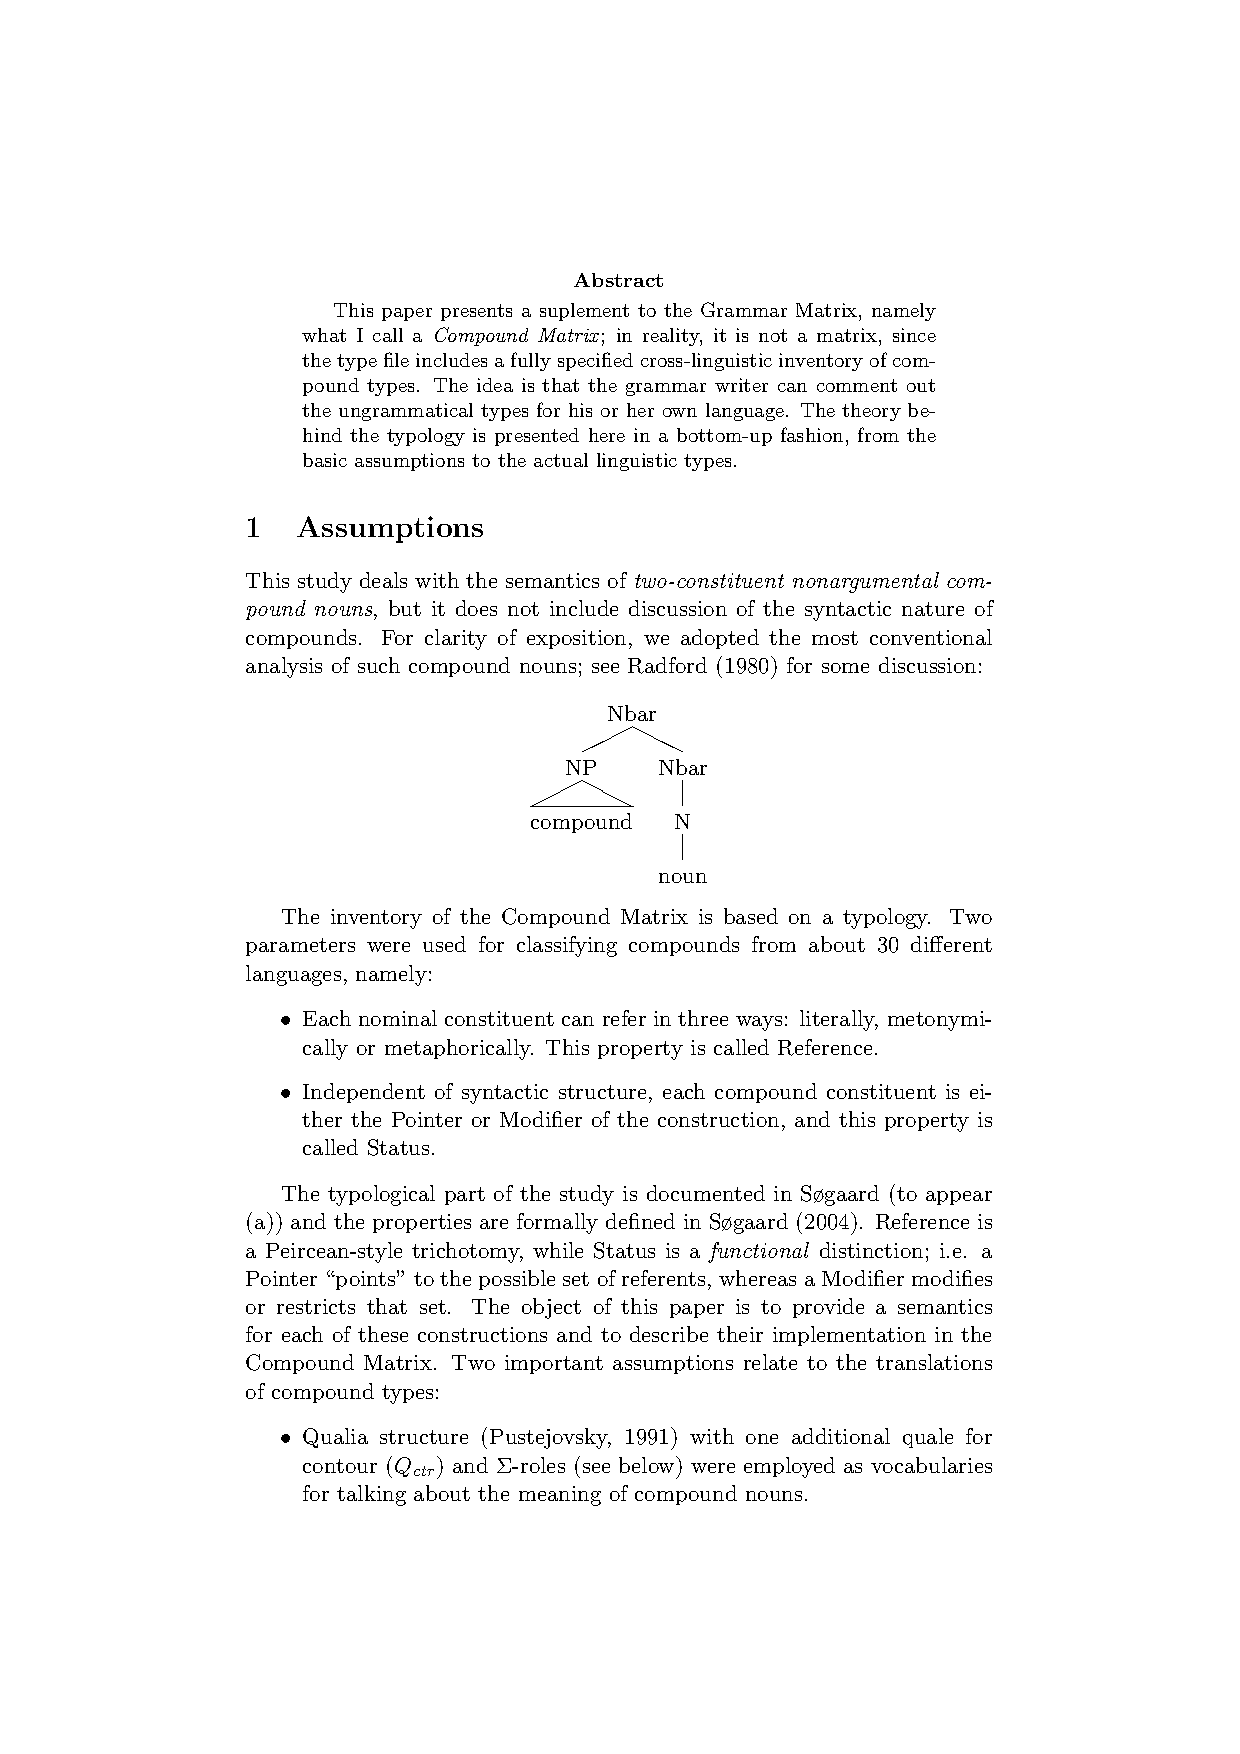
\includepdf[pages=-,pagecommand=\thispagestyle{plain}]{Includes/soegaard.pdf}
\end{document}
